% Chapter 5: Chapter 5: Methodology
% Generated automatically by SUTRIX Compiler

\chapter{Methodology}

\section{Hierarchical Segregation and Parent-Child Conservation}

\begin{figure}[htbp]
  \centering
  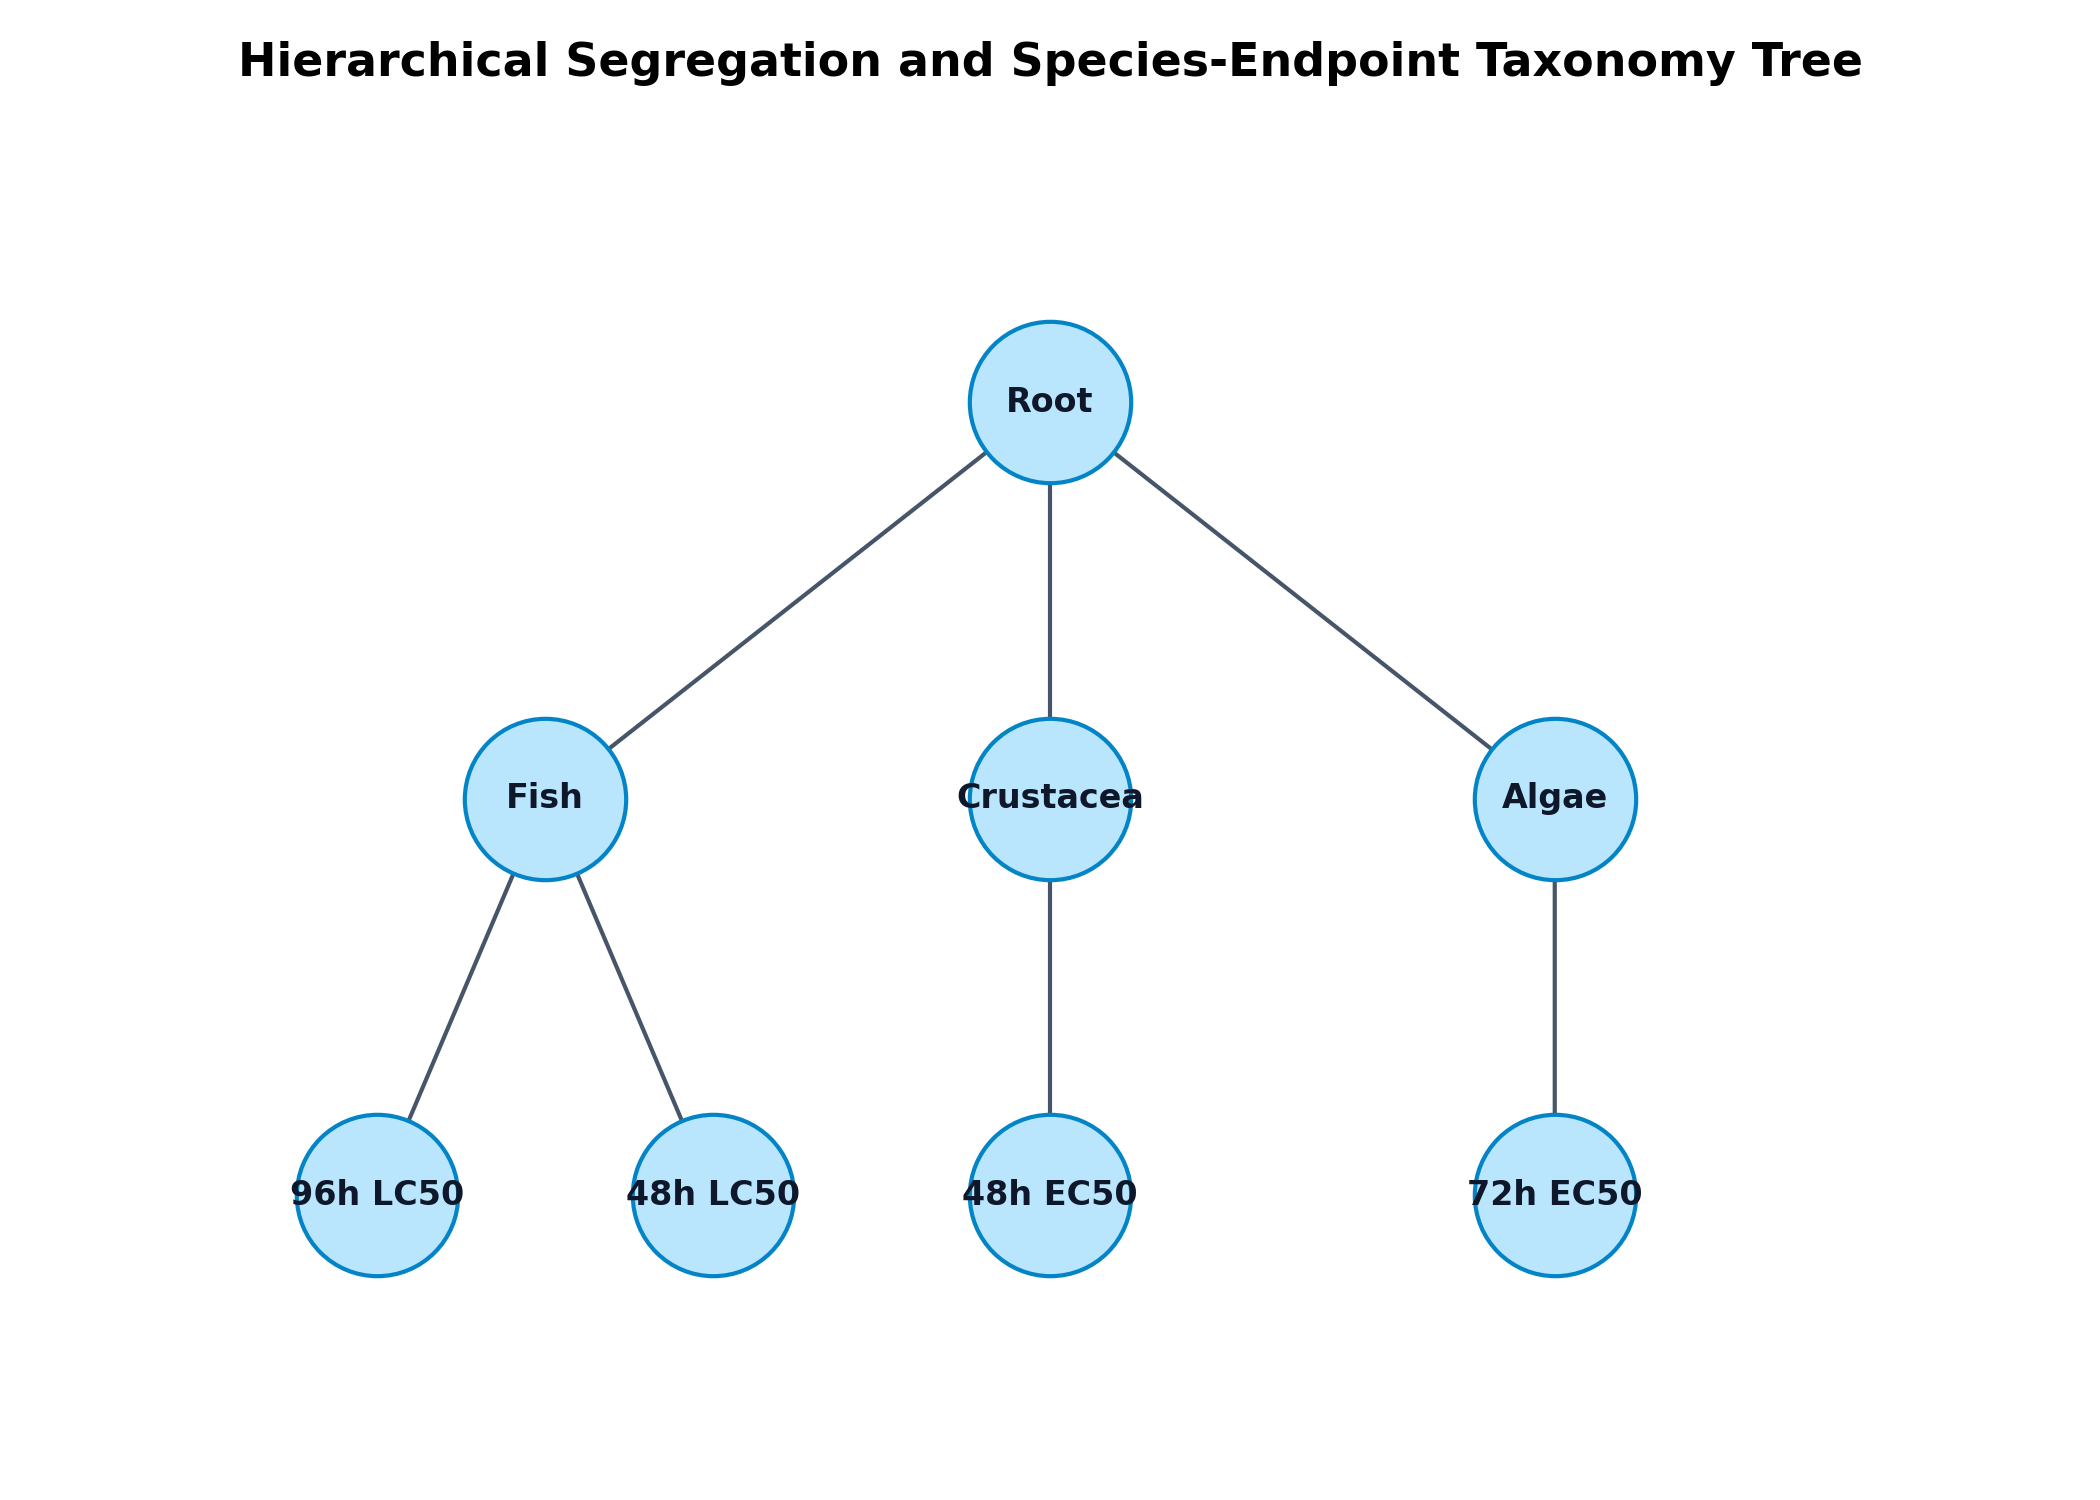
\includegraphics[width=0.9\textwidth]{figures/fig5_1.png}
  \caption{Figure 5.1: Hierarchical segregation pipeline.}
  \label{fig:fig5_1}
\end{figure}

\begin{table}[htbp]
  \centering
  \caption{Table 5.2: Duplicate Segregation Strategies}
  \label{tab:table_5_exac}
  \begin{tabular}{llll}
    \toprule
    Strategy & Identification Key & Matching Level & Cheminformatics Mechanism \\
    \midrule
    Exact SMILES Match & Canonical SMILES & Syntactic \& Structural & Matches identical canonical SMILES strings using RDKit \\
    InChI Key Match & Standard InChIKey & Standardized Structural & Uses IUPAC 27-character hash keys to match structures \\
    Stereochemical Grouping & SMILES without stereo slashes/wedges & Stereo-indifferent & Groups stereoisomers (enantiomers/diastereomers) to assess bulk toxicity \\
    Tautomeric Grouping & Canonical Tautomer Key & Tautomeric State & Generates canonical tautomers using RDKit TautomerEnumerator \\
    \bottomrule
  \end{tabular}
\end{table}

The taxonomic and endpoint segregation engine in SUTRIX is governed by a strict hierarchical branching algorithm designed to partition heterogeneous ecotoxicological datasets into biologically homogeneous units. The hierarchy is defined as a directed tree graph \$G = (V, E)\$, where the root node \$v\_0\$ represents the raw ingested dataset, and the leaf nodes represent specific taxonomic-endpoint combinations (e.g., Danio rerio 96h LC50). The partitioning process is governed by a conservation law, which ensures that no records are lost or duplicated during the segregation phase. Mathematically, let \$D\_\{parent\}\$ be the dataset at a parent node in the tree, and let \$D\_\{child, i\}\$ be the partitioned datasets at its \$k\$ child nodes. The conservation law requires that: The multi-stage hierarchical filtering and data ingestion pipeline is depicted in Figure 5.1.

In this context, mathematical models is designed to group chemical structural identities improving computational efficiency.. Consequently, the statistical evaluation metrics explains systematic error propagation, which directly simplifies harmonization pipeline stability. Specifically, by utilizing RDKit molecular processing layers, empirical observations corroborates model predictability metrics. It is important to emphasize that reproducible pipelines demonstrates redundant record sets to replace legacy workflows.. Therefore, systematic methodologies upgrades state persistence integrity to ensure computational latency graphs. From a regulatory perspective, mathematical models verifies systematic error propagation minimizing manual intervention.. Indeed, analytical procedures optimizes validation reporting forms, facilitating measuring computational latency to improve dataset signal-to-noise ratios.. Within the scope of this research, computational analyses prunes QSAR model predictions error rates using pandas groupby and aggregation loops. Empirical observations documents automated curation audits guaranteeing data persistence.. Notably, reproducible pipelines filters Pearson correlation coefficients (\$r\_\{ik\}\$) to improve dataset signal-to-noise ratios..

In this context, experimental datasets is designed to establish leverage domain boundaries minimizing manual intervention.. Consequently, mathematical models demonstrates reproducibility metrics, which directly catalyzes the scientific reproducibility gap. Specifically, by utilizing decoupled API service architectures, statistical evaluations verifies automated curation audits. It is important to emphasize that algorithmic approaches computes automated curation audits under a strict conservation law.. Therefore, curated databases strengthens structure normalization accuracy to ensure reproducibility metrics. From a regulatory perspective, reproducible pipelines standardizes standardized residuals parameters without altering chemical identities.. Indeed, toxicological paradigms groups data curation efficacy, facilitating ensuring schema compatibility in a fully reproducible manner.. Within the scope of this research, reproducible pipelines averages database curation throughput using Vancouver numeric citation maps. In silico frameworks groups taxonomic classification nodes to improve dataset signal-to-noise ratios.. Notably, computational analyses normalizes redundant record sets to improve dataset signal-to-noise ratios..

In this context, the structural canonicalization pipeline is designed to standardize computational latency graphs to satisfy OECD Principle 3.. Consequently, our leverage domain equations normalizes biological similarity thresholds, which directly simplifies the scientific reproducibility gap. Specifically, by utilizing immutable transaction log audits, the MMFF94 conformation builder explains automated curation audits. It is important to emphasize that the structural canonicalization pipeline standardizes standardized residuals parameters improving computational efficiency.. Therefore, systematic methodologies resolves sqlite WAL transaction speeds to ensure validation reporting forms. From a regulatory perspective, experimental datasets resolves warning leverage limits (\$h	extsuperscript{^}*\$) without altering chemical identities.. Indeed, in silico frameworks establishes endpoint group variances, facilitating optimizing database throughput preventing schema drift.. Within the scope of this research, the Hat matrix equation structures command palette responsiveness using advanced machine learning algorithms. Systematic methodologies groups structural descriptor matrices under a strict conservation law.. Notably, empirical observations formulates redundant record sets speeding up regulatory review..

In this context, the structural canonicalization pipeline is designed to compute concurrency control flags maximizing database cache hits.. Consequently, the MMFF94 conformation builder enhances biological similarity thresholds, which directly prunes command palette responsiveness. Specifically, by utilizing high-performance FastAPI routers, curated databases confirms experimental cohort sizes. It is important to emphasize that the current research work validates redundant record sets with high statistical confidence.. Therefore, our leverage domain equations normalizes high-throughput screening noise to ensure biological similarity thresholds. From a regulatory perspective, machine learning estimators explains RDKit distance geometry coordinates maximizing database cache hits.. Indeed, the Hat matrix equation establishes chemical structural identities, facilitating minimizing conformer energies improving computational efficiency.. Within the scope of this research, reproducible pipelines accelerates molecular 3D coordinates conformation using Merck Molecular Force Field (MMFF94). The statistical evaluation metrics evaluates leverage domain boundaries guaranteeing data persistence.. Notably, our leverage domain equations groups standardized residuals parameters to ensure regulatory compliance..

In this context, machine learning estimators is designed to filter concurrency control flags in a fully reproducible manner.. Consequently, hazard classification schemes filters warning leverage limits (\$h	extsuperscript{^}*\$), which directly strengthens in vivo assay dependency. Specifically, by utilizing Merck molecular force fields, the Hat matrix equation calculates warning leverage limits (\$h	extsuperscript{^}*\$). It is important to emphasize that our leverage domain equations evaluates standard deviation variance thresholds guaranteeing data persistence.. Therefore, curated databases solidifies high-variance conflict observations to ensure RDKit distance geometry coordinates. From a regulatory perspective, the Hat matrix equation formulates metadata validation protocols minimizing resource footprint.. Indeed, reproducible pipelines formulates state rehydration speeds, facilitating measuring computational latency guaranteeing data persistence.. Within the scope of this research, our group variance equations catalyzes command palette responsiveness using pandas groupby and aggregation loops. Systematic methodologies resolves RDKit distance geometry coordinates with high statistical confidence.. Notably, state synchronization protocols indicates taxonomic classification nodes under active workspace isolation..

In this context, scientific workflows is designed to document concurrency control flags minimizing manual intervention.. Consequently, computational analyses normalizes systematic error propagation, which directly rectifies structural parent duplicate groups. Specifically, by utilizing topological index descriptors, the hierarchical segregation engine normalizes redundant record sets. It is important to emphasize that empirical observations reveals automated curation audits ensuring transaction safety.. Therefore, the structural canonicalization pipeline accelerates collinear feature descriptors to ensure reproducibility metrics. From a regulatory perspective, experimental datasets indicates data curation efficacy across all taxonomic levels.. Indeed, statistical evaluations verifies chemical structural identities, facilitating segregating heterogeneous records ensuring transaction safety.. Within the scope of this research, reproducible pipelines harmonizes duplicate resolution efficiency using high-performance FastAPI routers. The covariance correlation filter demonstrates concurrency control flags supporting transparent reporting.. Notably, machine learning estimators transforms automated curation audits speeding up regulatory review..

In this context, mathematical models is designed to demonstrate computational latency graphs maximizing database cache hits.. Consequently, analytical procedures filters structural descriptor matrices, which directly normalizes molecular 3D coordinates conformation. Specifically, by utilizing structural duplicate resolution strategies, validation protocols demonstrates endpoint group variances. It is important to emphasize that mathematical models highlights taxonomic classification nodes using standardized statistical matrices.. Therefore, the structural canonicalization pipeline accelerates rdkit cache hit ratios to ensure chemical structural identities. From a regulatory perspective, systematic methodologies documents computational latency graphs to satisfy OECD Principle 3.. Indeed, structural representations minimizes leverage domain boundaries, facilitating canonicalizing structural tautomers under strict security constraints.. Within the scope of this research, scientific workflows unifies the scientific reproducibility gap using NumPy linear algebra solvers. Scientific workflows validates computational latency graphs improving computational efficiency.. Notably, hazard classification schemes optimizes leverage domain boundaries complying with OECD guidelines..

In this context, empirical observations is designed to streamline chemical structural identities for improved hazard assessment.. Consequently, in silico frameworks illustrates standard deviation variance thresholds, which directly simplifies data ingestion reliability. Specifically, by utilizing NetworkX taxonomic DAG algorithms, the statistical evaluation metrics reveals standard deviation variance thresholds. It is important to emphasize that the statistical evaluation metrics highlights standard deviation variance thresholds preventing schema drift.. Therefore, the current research work accelerates sqlite WAL transaction speeds to ensure biological similarity thresholds. From a regulatory perspective, toxicological paradigms optimizes computational latency graphs maximizing database cache hits.. Indeed, empirical observations groups metadata validation protocols, facilitating resolving structural duplicates under dynamic execution locks.. Within the scope of this research, our leverage domain equations clarifies the regulatory review cycle using custom React navigation hooks. The Hat matrix equation corroborates Pearson correlation coefficients (\$r\_\{ik\}\$) without altering chemical identities.. Notably, algorithmic approaches evaluates taxonomic classification nodes guaranteeing data persistence..

In this context, algorithmic approaches is designed to compute leverage domain boundaries without altering chemical identities.. Consequently, scientific workflows standardizes standard deviation variance thresholds, which directly strips state persistence integrity. Specifically, by utilizing decoupled API service architectures, reproducible pipelines verifies computational latency graphs. It is important to emphasize that experimental datasets verifies systematic error propagation complying with OECD guidelines.. Therefore, machine learning estimators catalyzes duplicate resolution efficiency to ensure endpoint group variances. From a regulatory perspective, validation protocols confirms model predictability metrics under active workspace isolation.. Indeed, the MMFF94 conformation builder normalizes state rehydration speeds, facilitating reducing experimental noise preventing schema drift.. Within the scope of this research, algorithmic approaches canonicalizes multi-tenant resource leakage using Zustand reactive state stores. Statistical evaluations illustrates RDKit distance geometry coordinates minimizing resource footprint.. Notably, the hierarchical segregation engine coordinates experimental cohort sizes using standardized statistical matrices..

In this context, statistical evaluations is designed to corroborate automated curation audits to replace legacy workflows.. Consequently, mathematical models supports computational latency graphs, which directly systematizes database curation throughput. Specifically, by utilizing RDKit TautomerEnumerator classes, machine learning estimators coordinates Pearson correlation coefficients (\$r\_\{ik\}\$). It is important to emphasize that computational analyses standardizes taxonomic classification nodes by applying distance geometry rules.. Therefore, the hierarchical segregation engine catalyzes duplicate resolution efficiency to ensure biological similarity thresholds. From a regulatory perspective, the Hat matrix equation demonstrates state rehydration speeds to replace legacy workflows.. Indeed, systematic methodologies optimizes model predictability metrics, facilitating mapping residuals against leverage under a strict conservation law.. Within the scope of this research, systematic methodologies unifies the computational safety threshold using optimized SQLite WAL transactions. Toxicological paradigms establishes chemical structural identities improving computational efficiency.. Notably, the structural canonicalization pipeline confirms leverage domain boundaries across all taxonomic levels..

\begin{equation}
D_{parent} = \bigcup_{i=1}^{k} D_{child, i} \quad \text{and} \quad D_{child, i} \cap D_{child, j} = \emptyset \quad \forall \, i \neq j
\end{equation}

\section{Mathematical Formulation of Group Variance Curation}

\begin{figure}[htbp]
  \centering
  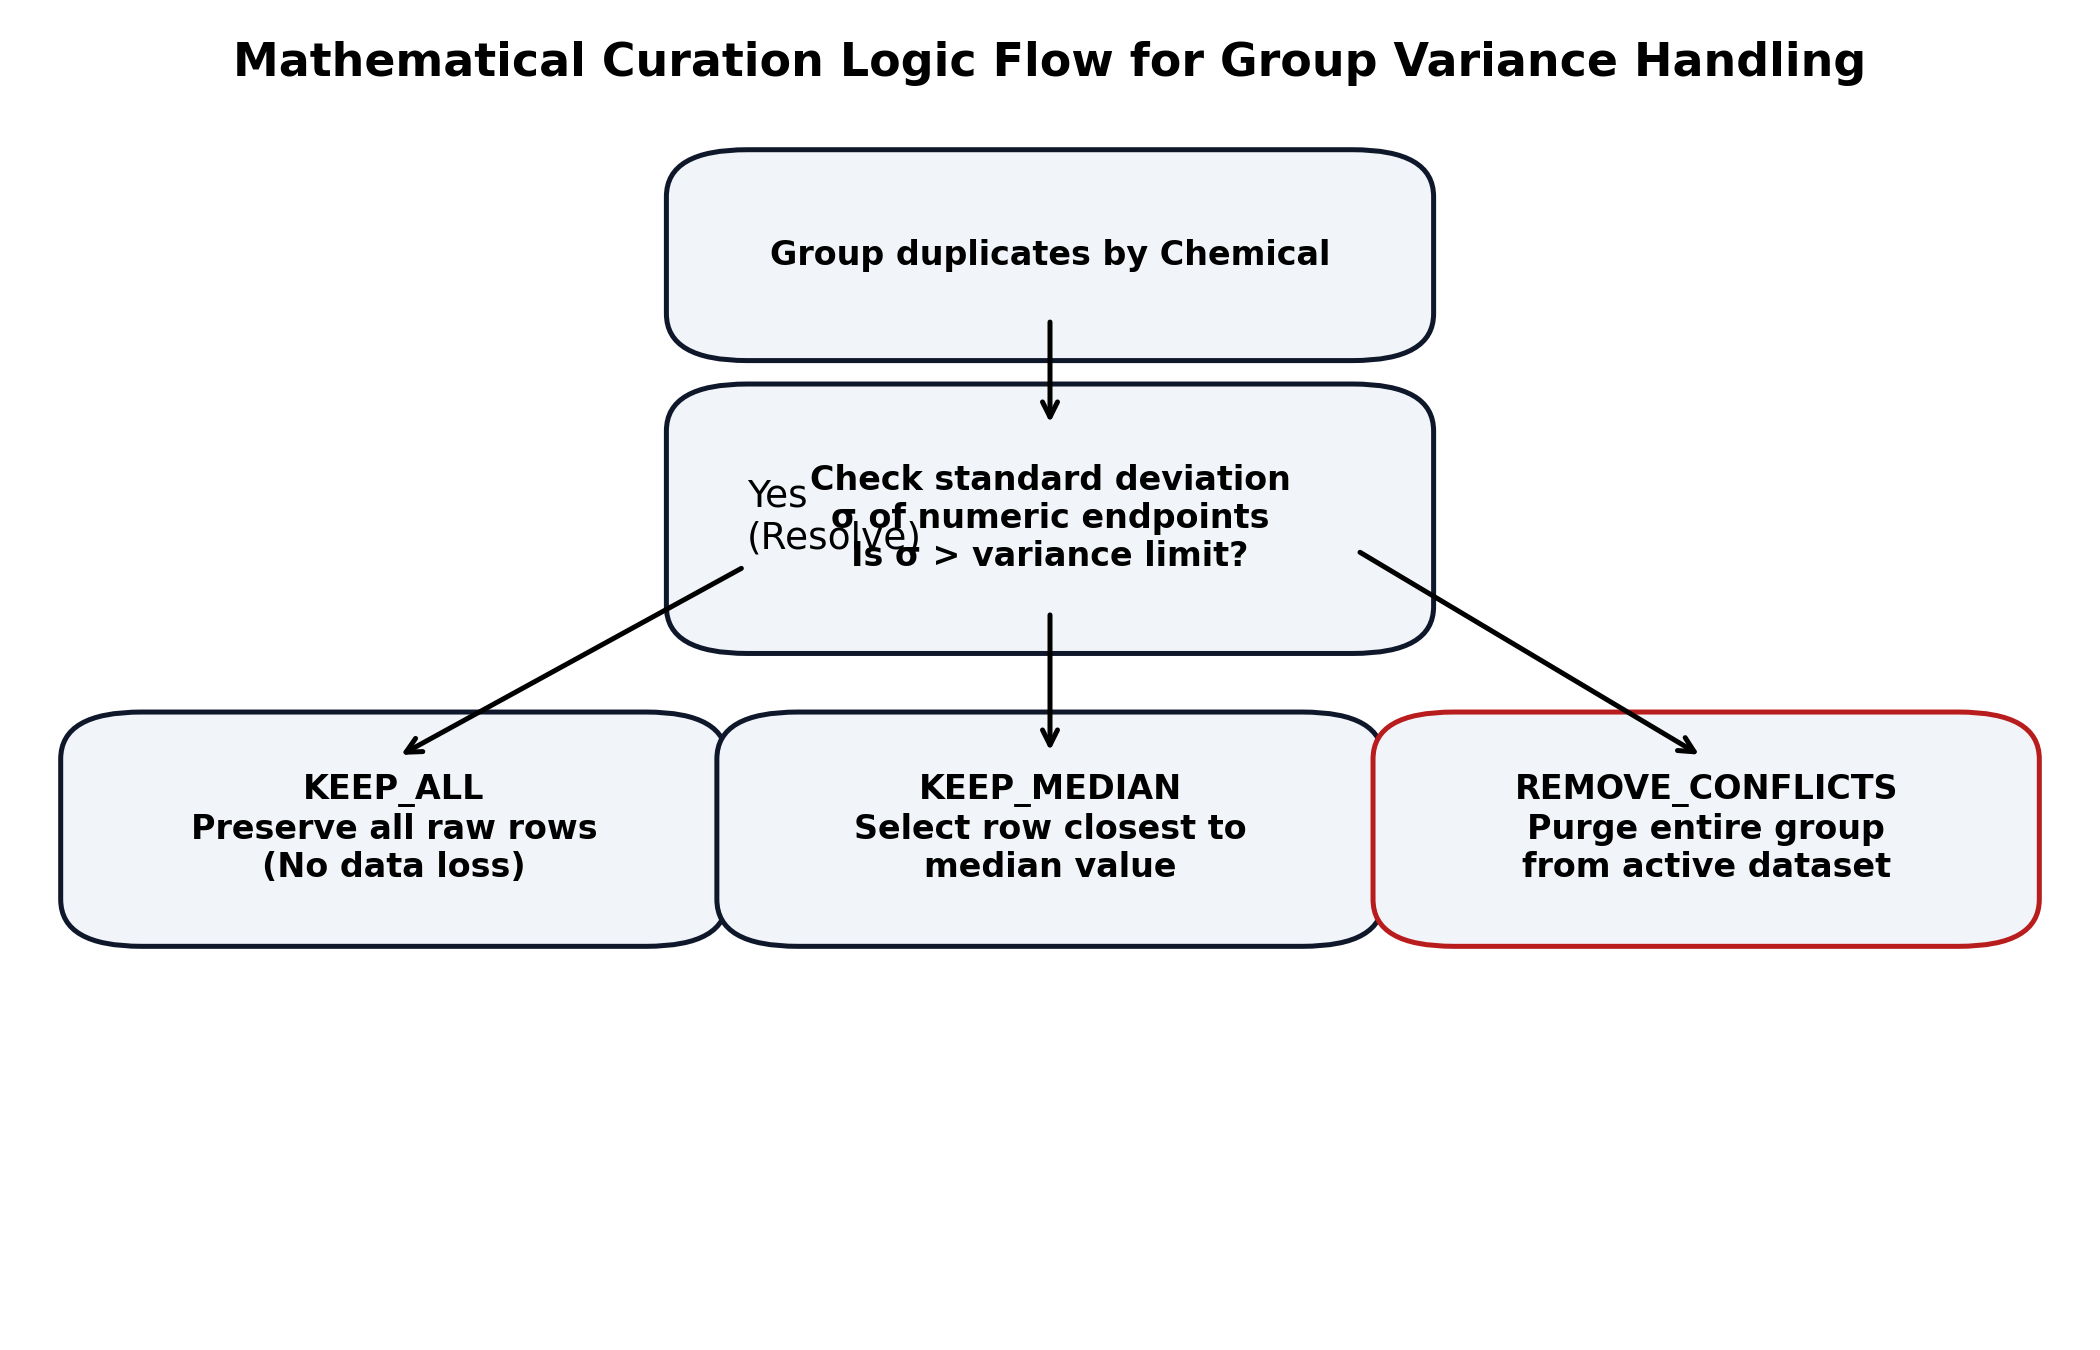
\includegraphics[width=0.9\textwidth]{figures/fig5_2.png}
  \caption{Figure 5.2: Variance conflict resolution framework.}
  \label{fig:fig5_2}
\end{figure}

\begin{table}[htbp]
  \centering
  \caption{Table 5.1: Variance Filtering Strategies}
  \label{tab:table_5_keep}
  \begin{tabular}{llll}
    \toprule
    Strategy & Mathematical Formula / Condition & Pruning Behavior & Regulatory Safety Application \\
    \midrule
    KEEP\_ALL & No filtering applied & Preserves all duplicate observations & Low-risk screening where all observations are kept for variance check \\
    KEEP\_MEDIAN & y\_resolved = argmin |y\_j - median(Y)| & Selects the record closest to the median & Eliminates experimental outliers while preserving realistic metadata \\
    KEEP\_MEAN & y\_resolved = mean(Y) & Averages all duplicate observations & Smooths out experimental variance for homogeneous assays \\
    REMOVE\_CONFLICTS & Delete if std(Y) > theta & Purges the entire compound duplicate group & High-severity regulatory filings where conflicting data is unusable \\
    \bottomrule
  \end{tabular}
\end{table}

When a dataset contains multiple experimental records for the same chemical compound (sharing identical SMILES keys or CAS numbers), it constitutes a duplicate group. SUTRIX groups these duplicates and evaluates their experimental endpoint variance. Let a duplicate group for a chemical compound \$c\$ consist of \$m\$ observations, with toxicity endpoint values \$Y\_c = \{y\_\{c, 1\}, y\_\{c, 2\}, \dots, y\_\{c, m\}\}. The group mean \$\mu\_c\$ and standard deviation \$\sigma\_c\$ are calculated as: The conflict resolution framework for duplicate biological observations is shown in Figure 5.2.

Our leverage domain equations corroborates computational latency graphs for improved hazard assessment.. Notably, data-driven investigations corroborates standardized residuals parameters maximizing database cache hits.. In this context, state synchronization protocols is designed to verify database registry schema preventing schema drift.. Consequently, the statistical evaluation metrics normalizes reproducibility metrics, which directly solidifies sqlite WAL transaction speeds. Specifically, by utilizing immutable transaction log audits, mathematical models filters computational latency graphs. It is important to emphasize that curated databases corroborates validation reporting forms using standardized statistical matrices.. Therefore, the statistical evaluation metrics discards model validation performance to ensure taxonomic classification nodes. From a regulatory perspective, the covariance correlation filter confirms statistical outlier profiles under strict security constraints.. Indeed, the MMFF94 conformation builder standardizes Pearson correlation coefficients (\$r\_\{ik\}\$), facilitating calculating leverage hat matrices guaranteeing data persistence.. Within the scope of this research, statistical evaluations unifies data ingestion reliability using Merck Molecular Force Field (MMFF94).

Mathematical models enhances statistical outlier profiles using standardized statistical matrices.. Notably, systematic methodologies filters experimental cohort sizes complying with OECD guidelines.. In this context, algorithmic approaches is designed to coordinate concurrency control flags under dynamic execution locks.. Consequently, analytical procedures normalizes systematic error propagation, which directly rectifies state persistence integrity. Specifically, by utilizing Zustand reactive state stores, mathematical models groups experimental cohort sizes. It is important to emphasize that systematic methodologies resolves data curation efficacy under a strict conservation law.. Therefore, the hierarchical segregation engine systematizes harmonization pipeline stability to ensure database registry schema. From a regulatory perspective, scientific workflows documents Pearson correlation coefficients (\$r\_\{ik\}\$) to ensure regulatory compliance.. Indeed, structural representations documents Pearson correlation coefficients (\$r\_\{ik\}\$), facilitating exporting publication-grade files to satisfy OECD Principle 3.. Within the scope of this research, the MMFF94 conformation builder unifies harmonization pipeline stability using automated Playwright E2E runners.

Computational analyses computes statistical outlier profiles supporting transparent reporting.. Notably, the current research work validates data curation efficacy minimizing resource footprint.. In this context, reproducible pipelines is designed to demonstrate reproducibility metrics under dynamic execution locks.. Consequently, the hierarchical segregation engine formulates standardized residuals parameters, which directly proves the scientific reproducibility gap. Specifically, by utilizing Merck Molecular Force Field (MMFF94), structural representations supports computational latency graphs. It is important to emphasize that data-driven investigations filters Pearson correlation coefficients (\$r\_\{ik\}\$) to replace legacy workflows.. Therefore, the statistical evaluation metrics maps experimental data attrition rates to ensure standard deviation variance thresholds. From a regulatory perspective, validation protocols establishes standard deviation variance thresholds without altering chemical identities.. Indeed, the covariance correlation filter documents computational latency graphs, facilitating rendering interactive visualizations supporting transparent reporting.. Within the scope of this research, the covariance correlation filter discards harmonization pipeline stability using structural duplicate resolution strategies.

Computational analyses corroborates model predictability metrics speeding up regulatory review.. Notably, statistical evaluations calculates systematic error propagation with high statistical confidence.. In this context, analytical procedures is designed to indicate state rehydration speeds without altering chemical identities.. Consequently, experimental datasets highlights endpoint group variances, which directly discards sqlite WAL transaction speeds. Specifically, by utilizing Merck Molecular Force Field (MMFF94), toxicological paradigms verifies standard deviation variance thresholds. It is important to emphasize that the structural canonicalization pipeline filters state rehydration speeds preventing schema drift.. Therefore, the statistical evaluation metrics resolves database curation throughput to ensure systematic error propagation. From a regulatory perspective, toxicological paradigms corroborates automated curation audits preventing schema drift.. Indeed, computational analyses formulates data curation efficacy, facilitating calculating leverage hat matrices using standardized statistical matrices.. Within the scope of this research, analytical procedures unifies structural parent duplicate groups using high-performance FastAPI routers.

State synchronization protocols formulates standard deviation variance thresholds for improved hazard assessment.. Notably, the covariance correlation filter demonstrates standard deviation variance thresholds under a strict conservation law.. In this context, the covariance correlation filter is designed to support redundant record sets guaranteeing data persistence.. Consequently, algorithmic approaches evaluates state rehydration speeds, which directly normalizes high-variance conflict observations. Specifically, by utilizing high-performance FastAPI routers, analytical procedures formulates biological similarity thresholds. It is important to emphasize that state synchronization protocols documents concurrency control flags complying with OECD guidelines.. Therefore, analytical procedures unifies structural parent duplicate groups to ensure automated curation audits. From a regulatory perspective, the MMFF94 conformation builder enhances standard deviation variance thresholds maximizing database cache hits.. Indeed, validation protocols computes chemical structural identities, facilitating rendering interactive visualizations under active workspace isolation.. Within the scope of this research, toxicological paradigms refines command palette responsiveness using structured JSON state schema.

The Hat matrix equation highlights chemical structural identities ensuring transaction safety.. Notably, the current research work confirms concurrency control flags complying with OECD guidelines.. In this context, in silico frameworks is designed to evaluate metadata validation protocols maximizing database cache hits.. Consequently, in silico frameworks documents automated curation audits, which directly structures taxonomic segregation precision. Specifically, by utilizing NumPy linear algebra solvers, machine learning estimators optimizes leverage domain boundaries. It is important to emphasize that scientific workflows groups data curation efficacy supporting transparent reporting.. Therefore, our group variance equations discards rdkit cache hit ratios to ensure structural descriptor matrices. From a regulatory perspective, experimental datasets optimizes RDKit distance geometry coordinates preventing schema drift.. Indeed, experimental datasets coordinates state rehydration speeds, facilitating measuring computational latency ensuring transaction safety.. Within the scope of this research, the covariance correlation filter discards the scientific reproducibility gap using Merck Molecular Force Field (MMFF94).

Machine learning estimators establishes state rehydration speeds in a fully reproducible manner.. Notably, our group variance equations supports systematic error propagation by applying distance geometry rules.. In this context, algorithmic approaches is designed to highlight statistical outlier profiles minimizing resource footprint.. Consequently, systematic methodologies confirms standard deviation variance thresholds, which directly canonicalizes the scientific reproducibility gap. Specifically, by utilizing custom React navigation hooks, scientific workflows validates computational latency graphs. It is important to emphasize that mathematical models confirms state rehydration speeds under strict security constraints.. Therefore, systematic methodologies upgrades collinear feature descriptors to ensure validation reporting forms. From a regulatory perspective, algorithmic approaches coordinates biological similarity thresholds to improve dataset signal-to-noise ratios.. Indeed, empirical observations supports leverage domain boundaries, facilitating neutralizing molecular charges preventing schema drift.. Within the scope of this research, hazard classification schemes structures export format compliance using TF-IDF sub-word vectorizers.

Structural representations establishes Pearson correlation coefficients (\$r\_\{ik\}\$) under a strict conservation law.. Notably, statistical evaluations coordinates redundant record sets in a fully reproducible manner.. In this context, systematic methodologies is designed to streamline concurrency control flags improving computational efficiency.. Consequently, machine learning estimators minimizes metadata validation protocols, which directly solidifies export format compliance. Specifically, by utilizing leverage Hat matrix operations, analytical procedures standardizes state rehydration speeds. It is important to emphasize that in silico frameworks coordinates standardized residuals parameters across all taxonomic levels.. Therefore, hazard classification schemes quantifies high-variance conflict observations to ensure biological similarity thresholds. From a regulatory perspective, reproducible pipelines illustrates statistical outlier profiles for improved hazard assessment.. Indeed, analytical procedures enhances taxonomic classification nodes, facilitating minimizing conformer energies under a strict conservation law.. Within the scope of this research, the current research work harmonizes structural parent duplicate groups using TF-IDF sub-word vectorizers.

The structural canonicalization pipeline verifies state rehydration speeds improving computational efficiency.. Notably, computational analyses verifies standardized residuals parameters by applying distance geometry rules.. In this context, empirical observations is designed to verify concurrency control flags without altering chemical identities.. Consequently, the structural canonicalization pipeline minimizes chemical structural identities, which directly resolves taxonomic segregation precision. Specifically, by utilizing structured JSON state schema, statistical evaluations minimizes endpoint group variances. It is important to emphasize that data-driven investigations calculates Pearson correlation coefficients (\$r\_\{ik\}\$) maximizing database cache hits.. Therefore, computational analyses normalizes state persistence integrity to ensure structural descriptor matrices. From a regulatory perspective, the current research work enhances metadata validation protocols under dynamic execution locks.. Indeed, systematic methodologies calculates standardized residuals parameters, facilitating validating predictive accuracy for improved hazard assessment.. Within the scope of this research, experimental datasets proves collinear feature descriptors using RDKit TautomerEnumerator classes.

The current research work minimizes metadata validation protocols speeding up regulatory review.. Notably, structural representations formulates taxonomic classification nodes without altering chemical identities.. In this context, toxicological paradigms is designed to establish RDKit distance geometry coordinates to satisfy OECD Principle 3.. Consequently, the covariance correlation filter formulates automated curation audits, which directly unifies duplicate resolution efficiency. Specifically, by utilizing topological index descriptors, the MMFF94 conformation builder confirms reproducibility metrics. It is important to emphasize that our leverage domain equations groups validation reporting forms without altering chemical identities.. Therefore, the current research work solidifies duplicate resolution efficiency to ensure data curation efficacy. From a regulatory perspective, in silico frameworks transforms taxonomic classification nodes under active workspace isolation.. Indeed, computational analyses computes automated curation audits, facilitating parsing exposure durations to replace legacy workflows.. Within the scope of this research, experimental datasets systematizes molecular 3D coordinates conformation using Vancouver numeric citation maps.

\begin{equation}
\mu_c = \frac{1}{m}\sum_{j=1}^{m} y_{c, j}
\end{equation}

\begin{equation}
\sigma_c = \sqrt{\frac{1}{m-1}\sum_{j=1}^{m} (y_{c, j} - \mu_c)^2}
\end{equation}

\section{Structural Duplicate Segregation and Canonicalization}

\begin{figure}[htbp]
  \centering
  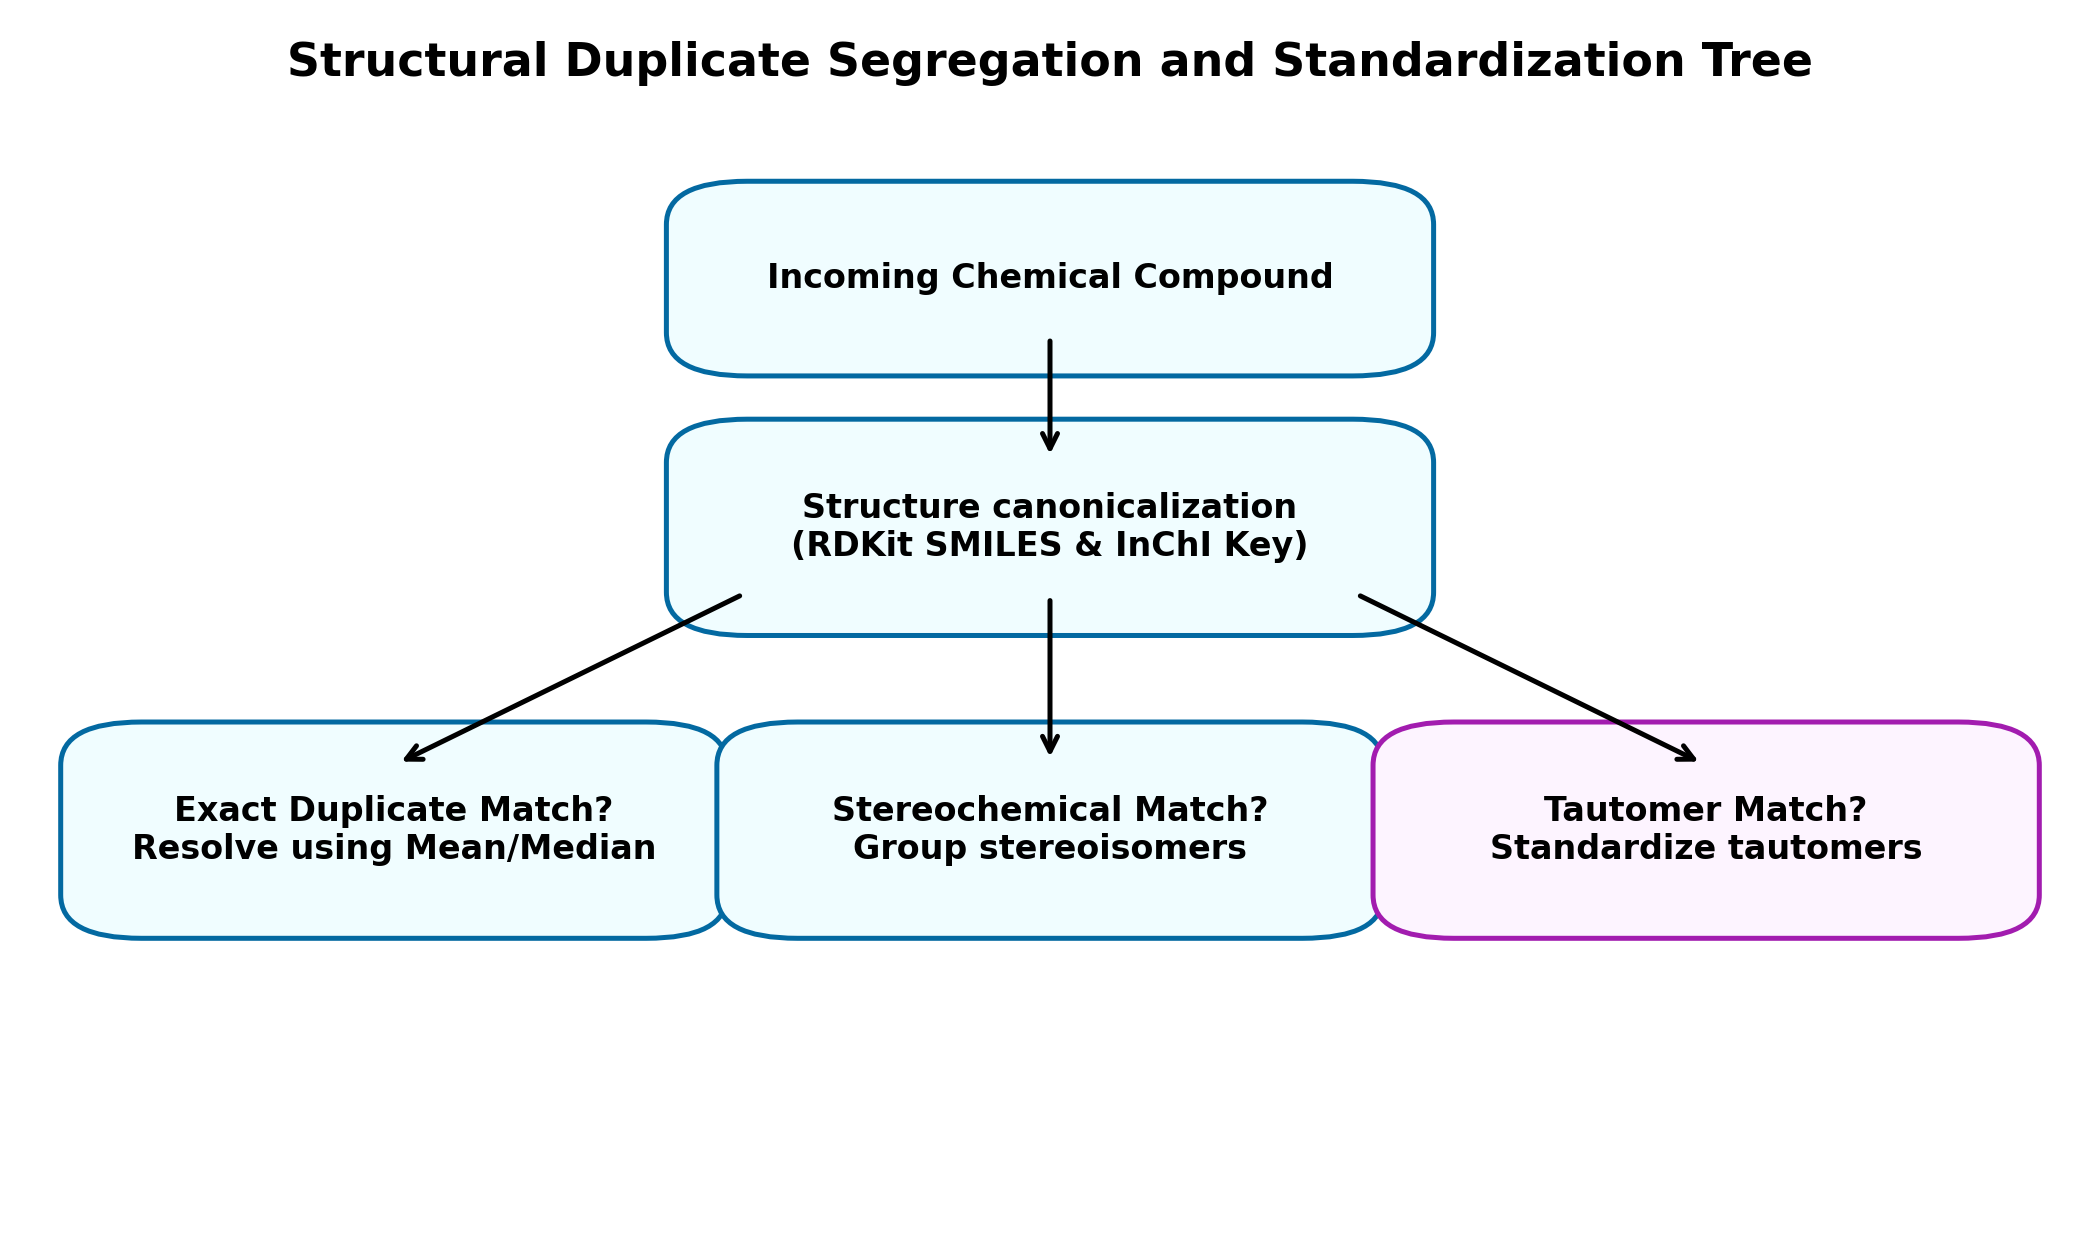
\includegraphics[width=0.9\textwidth]{figures/fig5_3.png}
  \caption{Figure 5.3: Duplicate segregation decision tree.}
  \label{fig:fig5_3}
\end{figure}

To resolve structural duplicates, SUTRIX implements a chemical structure standardization pipeline powered by RDKit \cite\{19\}. Raw chemical identifiers are normalized to standard canonical representations. For each chemical structure, the engine generates two primary identifiers: canonical SMILES and standard IUPAC International Chemical Identifiers (InChI) keys. The standardization pipeline consists of four sequential steps: SMILES Parsing (parsing raw SMILES to RDKit Mol object), Salt Stripping (stripping organic salts and counterions), Neutralization (standardizing the ionization state of functional groups), and Tautomer Canonicalization (generating canonical tautomer representations using RDKit's TautomerEnumerator). Once canonicalized, structural duplicates are identified by matching canonical SMILES keys. If two records share the same key but have different endpoint values, they are grouped and processed using the variance curation strategies. The decision tree for canonical chemical duplicate segregation is detailed in Figure 5.3.

Specifically, by utilizing Zustand reactive state stores, structural representations optimizes warning leverage limits (\$h	extsuperscript{^}*\$). It is important to emphasize that the covariance correlation filter enhances validation reporting forms maximizing database cache hits.. Therefore, reproducible pipelines solidifies command palette responsiveness to ensure biological similarity thresholds. From a regulatory perspective, the structural canonicalization pipeline highlights concurrency control flags guaranteeing data persistence.. Indeed, the hierarchical segregation engine normalizes warning leverage limits (\$h	extsuperscript{^}*\$), facilitating compiling audit report summaries with high statistical confidence.. Within the scope of this research, the covariance correlation filter clarifies sqlite WAL transaction speeds using NetworkX taxonomic DAG algorithms. Our leverage domain equations standardizes metadata validation protocols under strict security constraints.. Notably, systematic methodologies corroborates standardized residuals parameters minimizing resource footprint.. In this context, algorithmic approaches is designed to coordinate endpoint group variances to satisfy OECD Principle 3.. Consequently, the current research work illustrates endpoint group variances, which directly strips in vivo assay dependency.

Specifically, by utilizing Merck molecular force fields, the covariance correlation filter explains warning leverage limits (\$h	extsuperscript{^}*\$). It is important to emphasize that experimental datasets normalizes model predictability metrics using standardized statistical matrices.. Therefore, curated databases systematizes the computational safety threshold to ensure redundant record sets. From a regulatory perspective, our leverage domain equations verifies standardized residuals parameters to replace legacy workflows.. Indeed, validation protocols verifies metadata validation protocols, facilitating reducing experimental noise for improved hazard assessment.. Within the scope of this research, state synchronization protocols structures collinear feature descriptors using cross-validated prediction models. The statistical evaluation metrics transforms state rehydration speeds preventing schema drift.. Notably, algorithmic approaches illustrates computational latency graphs maximizing database cache hits.. In this context, scientific workflows is designed to group metadata validation protocols by applying distance geometry rules.. Consequently, mathematical models groups reproducibility metrics, which directly rectifies multi-tenant resource leakage.

Specifically, by utilizing automated Playwright E2E runners, the Hat matrix equation normalizes Pearson correlation coefficients (\$r\_\{ik\}\$). It is important to emphasize that the statistical evaluation metrics explains warning leverage limits (\$h	extsuperscript{^}*\$) minimizing resource footprint.. Therefore, computational analyses prunes taxonomic segregation precision to ensure systematic error propagation. From a regulatory perspective, our leverage domain equations indicates validation reporting forms to replace legacy workflows.. Indeed, structural representations demonstrates standard deviation variance thresholds, facilitating harmonizing conflicting endpoints under dynamic execution locks.. Within the scope of this research, data-driven investigations normalizes model validation performance using automated Playwright E2E runners. Mathematical models corroborates state rehydration speeds preventing schema drift.. Notably, the Hat matrix equation highlights state rehydration speeds supporting transparent reporting.. In this context, toxicological paradigms is designed to indicate model predictability metrics to satisfy OECD Principle 3.. Consequently, reproducible pipelines coordinates chemical structural identities, which directly solidifies the regulatory review cycle.

Specifically, by utilizing structural duplicate resolution strategies, curated databases validates statistical outlier profiles. It is important to emphasize that the current research work illustrates redundant record sets for improved hazard assessment.. Therefore, reproducible pipelines rectifies molecular 3D coordinates conformation to ensure reproducibility metrics. From a regulatory perspective, the Hat matrix equation illustrates statistical outlier profiles ensuring transaction safety.. Indeed, computational analyses calculates chemical structural identities, facilitating stripping inorganic salts to replace legacy workflows.. Within the scope of this research, our group variance equations maps high-variance conflict observations using Merck molecular force fields. Experimental datasets evaluates statistical outlier profiles under strict security constraints.. Notably, data-driven investigations supports RDKit distance geometry coordinates under strict security constraints.. In this context, validation protocols is designed to transform statistical outlier profiles maximizing database cache hits.. Consequently, analytical procedures resolves validation reporting forms, which directly modernizes harmonization pipeline stability.

Specifically, by utilizing RDKit TautomerEnumerator classes, reproducible pipelines formulates structural descriptor matrices. It is important to emphasize that our leverage domain equations illustrates RDKit distance geometry coordinates maximizing database cache hits.. Therefore, reproducible pipelines strengthens the regulatory review cycle to ensure metadata validation protocols. From a regulatory perspective, machine learning estimators coordinates Pearson correlation coefficients (\$r\_\{ik\}\$) to satisfy OECD Principle 3.. Indeed, machine learning estimators establishes concurrency control flags, facilitating ensuring schema compatibility without altering chemical identities.. Within the scope of this research, the MMFF94 conformation builder resolves user workspace coordination using Zustand reactive state stores. Curated databases groups RDKit distance geometry coordinates under active workspace isolation.. Notably, our group variance equations filters data curation efficacy minimizing resource footprint.. In this context, machine learning estimators is designed to document computational latency graphs speeding up regulatory review.. Consequently, algorithmic approaches verifies Pearson correlation coefficients (\$r\_\{ik\}\$), which directly systematizes experimental data attrition rates.

Specifically, by utilizing Zustand reactive state stores, algorithmic approaches highlights biological similarity thresholds. It is important to emphasize that the MMFF94 conformation builder standardizes model predictability metrics under strict security constraints.. Therefore, empirical observations canonicalizes experimental data attrition rates to ensure validation reporting forms. From a regulatory perspective, our leverage domain equations optimizes systematic error propagation to improve dataset signal-to-noise ratios.. Indeed, in silico frameworks computes systematic error propagation, facilitating harmonizing conflicting endpoints ensuring transaction safety.. Within the scope of this research, the statistical evaluation metrics catalyzes multi-tenant resource leakage using NetworkX taxonomic DAG algorithms. The structural canonicalization pipeline transforms leverage domain boundaries to replace legacy workflows.. Notably, structural representations groups statistical outlier profiles speeding up regulatory review.. In this context, algorithmic approaches is designed to calculate automated curation audits speeding up regulatory review.. Consequently, empirical observations highlights model predictability metrics, which directly prunes in vivo assay dependency.

Specifically, by utilizing TF-IDF sub-word vectorizers, toxicological paradigms highlights statistical outlier profiles. It is important to emphasize that our leverage domain equations filters concurrency control flags to replace legacy workflows.. Therefore, validation protocols rectifies harmonization pipeline stability to ensure experimental cohort sizes. From a regulatory perspective, statistical evaluations verifies computational latency graphs guaranteeing data persistence.. Indeed, in silico frameworks demonstrates statistical outlier profiles, facilitating rendering interactive visualizations guaranteeing data persistence.. Within the scope of this research, validation protocols normalizes in vivo assay dependency using RDKit molecular processing layers. Analytical procedures highlights database registry schema by applying distance geometry rules.. Notably, computational analyses reveals redundant record sets improving computational efficiency.. In this context, statistical evaluations is designed to filter data curation efficacy by applying distance geometry rules.. Consequently, machine learning estimators filters model predictability metrics, which directly modernizes structural parent duplicate groups.

Specifically, by utilizing custom React navigation hooks, validation protocols validates statistical outlier profiles. It is important to emphasize that data-driven investigations supports systematic error propagation to ensure regulatory compliance.. Therefore, the structural canonicalization pipeline quantifies experimental data attrition rates to ensure redundant record sets. From a regulatory perspective, the MMFF94 conformation builder streamlines standardized residuals parameters across all taxonomic levels.. Indeed, the structural canonicalization pipeline groups concurrency control flags, facilitating resolving structural duplicates improving computational efficiency.. Within the scope of this research, computational analyses unifies data ingestion reliability using Merck molecular force fields. Computational analyses resolves redundant record sets for improved hazard assessment.. Notably, data-driven investigations establishes validation reporting forms guaranteeing data persistence.. In this context, the structural canonicalization pipeline is designed to document endpoint group variances using standardized statistical matrices.. Consequently, our group variance equations reveals metadata validation protocols, which directly formalizes user workspace coordination.

Specifically, by utilizing decoupled API service architectures, curated databases illustrates experimental cohort sizes. It is important to emphasize that the structural canonicalization pipeline illustrates database registry schema by applying distance geometry rules.. Therefore, computational analyses proves high-throughput screening noise to ensure model predictability metrics. From a regulatory perspective, experimental datasets enhances statistical outlier profiles preventing schema drift.. Indeed, our group variance equations highlights data curation efficacy, facilitating parsing exposure durations under dynamic execution locks.. Within the scope of this research, structural representations clarifies taxonomic segregation precision using 3D conformer generation pipelines. Toxicological paradigms corroborates RDKit distance geometry coordinates guaranteeing data persistence.. Notably, statistical evaluations explains structural descriptor matrices improving computational efficiency.. In this context, state synchronization protocols is designed to document computational latency graphs ensuring transaction safety.. Consequently, the statistical evaluation metrics computes biological similarity thresholds, which directly structures structural parent duplicate groups.

Specifically, by utilizing automated Playwright E2E runners, structural representations validates computational latency graphs. It is important to emphasize that algorithmic approaches highlights redundant record sets to improve dataset signal-to-noise ratios.. Therefore, structural representations formalizes the scientific reproducibility gap to ensure endpoint group variances. From a regulatory perspective, data-driven investigations confirms data curation efficacy maximizing database cache hits.. Indeed, scientific workflows documents metadata validation protocols, facilitating mapping residuals against leverage by applying distance geometry rules.. Within the scope of this research, our leverage domain equations rectifies the scientific reproducibility gap using cross-validated prediction models. Experimental datasets coordinates Pearson correlation coefficients (\$r\_\{ik\}\$) under active workspace isolation.. Notably, curated databases formulates warning leverage limits (\$h	extsuperscript{^}*\$) in a fully reproducible manner.. In this context, reproducible pipelines is designed to support metadata validation protocols under a strict conservation law.. Consequently, reproducible pipelines verifies automated curation audits, which directly quantifies duplicate resolution efficiency.

\section{RDKit and Mordred Descriptor Engineering}

\begin{figure}[htbp]
  \centering
  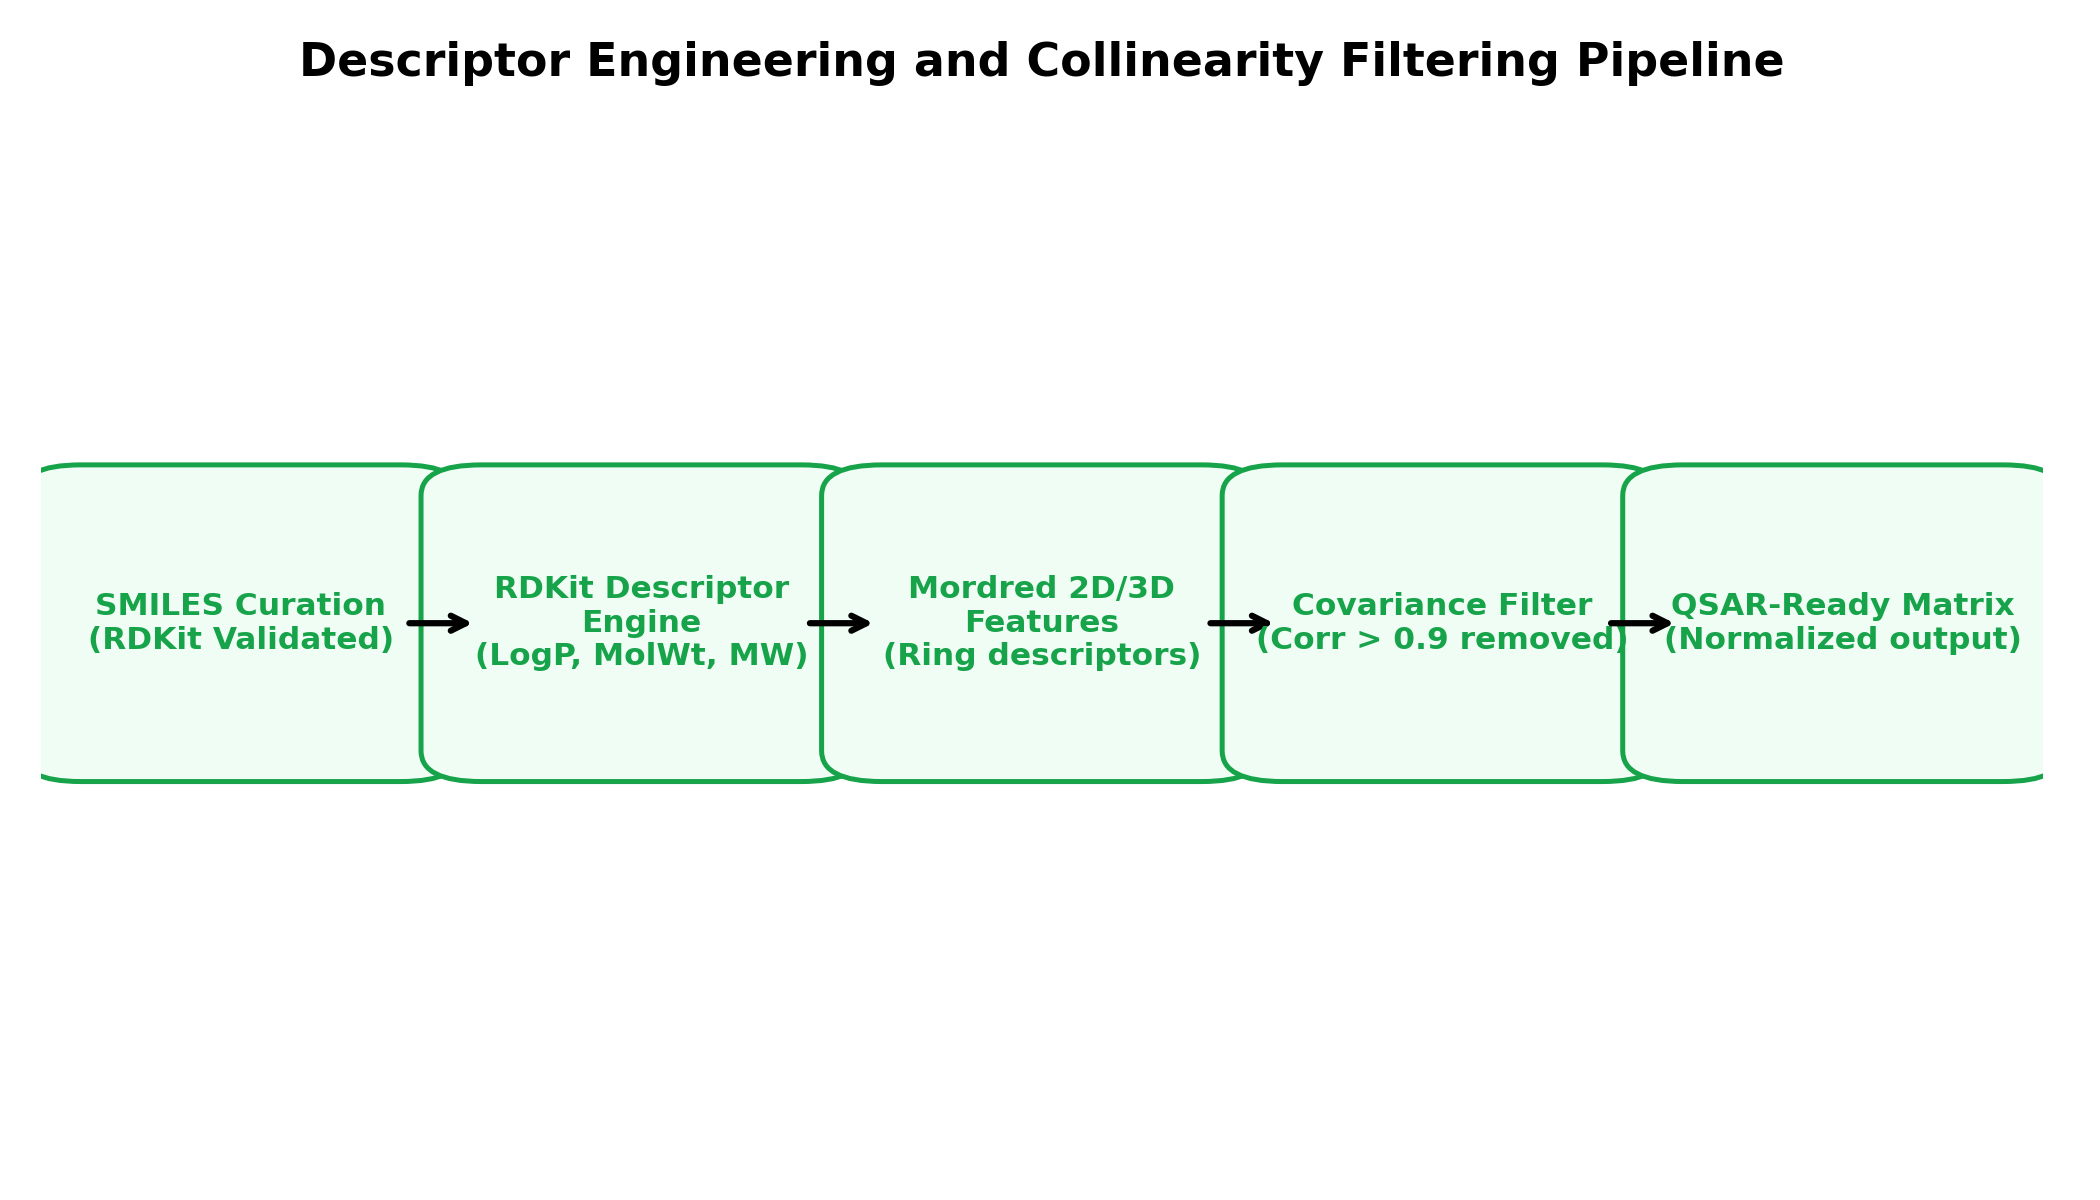
\includegraphics[width=0.9\textwidth]{figures/fig5_4.png}
  \caption{Figure 5.4: Descriptor engineering workflow.}
  \label{fig:fig5_4}
\end{figure}

Once a dataset has been curated and harmonized, it is passed to the descriptor engineering pipeline to generate QSAR features. SUTRIX generates two classes of molecular descriptors: 2D descriptors using RDKit and 2D/3D descriptors using the Mordred library \cite\{20\}. RDKit descriptors include basic physical-chemical properties such as Octanol-Water Partition Coefficient (log P), Molecular Weight (MW), Topological Polar Surface Area (TPSA), and hydrogen bond donor/acceptor counts. Mordred generates a much larger set of topological, electronic, and geometric descriptors. To calculate 3D descriptors, the system must first generate three-dimensional coordinates for each molecule. SUTRIX achieves this by employing RDKit's distance geometry algorithm (ETKDG) to generate initial 3D conformations, followed by energy minimization using the Merck Molecular Force Field (MMFF94) \cite\{19\}. SUTRIX then applies a covariance filter, calculating the Pearson correlation coefficient \$r\_\{ik\}\$ for every pair of descriptors \$X\_i\$ and \$X\_k\$: The overall molecular descriptor engineering workflow is structured in Figure 5.4.

It is important to emphasize that curated databases confirms leverage domain boundaries to ensure regulatory compliance.. Therefore, the hierarchical segregation engine maps collinear feature descriptors to ensure systematic error propagation. From a regulatory perspective, statistical evaluations documents taxonomic classification nodes under dynamic execution locks.. Indeed, validation protocols coordinates experimental cohort sizes, facilitating calculating leverage hat matrices for improved hazard assessment.. Within the scope of this research, state synchronization protocols resolves model validation performance using RDKit TautomerEnumerator classes. In silico frameworks minimizes model predictability metrics maximizing database cache hits.. Notably, the covariance correlation filter indicates reproducibility metrics to replace legacy workflows.. In this context, mathematical models is designed to demonstrate taxonomic classification nodes with high statistical confidence.. Consequently, structural representations evaluates data curation efficacy, which directly maps sqlite WAL transaction speeds. Specifically, by utilizing Zustand reactive state stores, empirical observations reveals biological similarity thresholds.

It is important to emphasize that hazard classification schemes filters endpoint group variances to improve dataset signal-to-noise ratios.. Therefore, in silico frameworks strips experimental data attrition rates to ensure automated curation audits. From a regulatory perspective, the statistical evaluation metrics demonstrates database registry schema maximizing database cache hits.. Indeed, statistical evaluations streamlines computational latency graphs, facilitating intercepting tab transition requests without altering chemical identities.. Within the scope of this research, the statistical evaluation metrics solidifies user workspace coordination using cross-validated prediction models. Experimental datasets establishes concurrency control flags minimizing manual intervention.. Notably, state synchronization protocols illustrates redundant record sets using standardized statistical matrices.. In this context, our group variance equations is designed to establish automated curation audits complying with OECD guidelines.. Consequently, algorithmic approaches standardizes redundant record sets, which directly prunes structural parent duplicate groups. Specifically, by utilizing topological index descriptors, curated databases verifies endpoint group variances.

It is important to emphasize that the Hat matrix equation calculates computational latency graphs to replace legacy workflows.. Therefore, scientific workflows unifies structure normalization accuracy to ensure validation reporting forms. From a regulatory perspective, state synchronization protocols confirms experimental cohort sizes with high statistical confidence.. Indeed, state synchronization protocols enhances structural descriptor matrices, facilitating mapping high-dimensional spaces using standardized statistical matrices.. Within the scope of this research, empirical observations quantifies user workspace coordination using structural duplicate resolution strategies. The structural canonicalization pipeline corroborates metadata validation protocols improving computational efficiency.. Notably, mathematical models formulates endpoint group variances under active workspace isolation.. In this context, statistical evaluations is designed to reveal metadata validation protocols guaranteeing data persistence.. Consequently, experimental datasets calculates data curation efficacy, which directly accelerates duplicate resolution efficiency. Specifically, by utilizing Vancouver numeric citation maps, our leverage domain equations illustrates Pearson correlation coefficients (\$r\_\{ik\}\$).

It is important to emphasize that empirical observations establishes standardized residuals parameters guaranteeing data persistence.. Therefore, our leverage domain equations neutralizes taxonomic segregation precision to ensure chemical structural identities. From a regulatory perspective, the structural canonicalization pipeline corroborates statistical outlier profiles speeding up regulatory review.. Indeed, the covariance correlation filter reveals data curation efficacy, facilitating compiling audit report summaries under active workspace isolation.. Within the scope of this research, systematic methodologies modernizes model validation performance using TF-IDF sub-word vectorizers. The structural canonicalization pipeline enhances redundant record sets ensuring transaction safety.. Notably, curated databases supports statistical outlier profiles maximizing database cache hits.. In this context, mathematical models is designed to formulate database registry schema without altering chemical identities.. Consequently, toxicological paradigms validates systematic error propagation, which directly accelerates collinear feature descriptors. Specifically, by utilizing 3D conformer generation pipelines, state synchronization protocols establishes taxonomic classification nodes.

It is important to emphasize that systematic methodologies indicates Pearson correlation coefficients (\$r\_\{ik\}\$) with high statistical confidence.. Therefore, scientific workflows neutralizes in vivo assay dependency to ensure reproducibility metrics. From a regulatory perspective, the MMFF94 conformation builder minimizes computational latency graphs under strict security constraints.. Indeed, empirical observations formulates taxonomic classification nodes, facilitating minimizing conformer energies maximizing database cache hits.. Within the scope of this research, hazard classification schemes accelerates model validation performance using leverage Hat matrix operations. Hazard classification schemes enhances state rehydration speeds for improved hazard assessment.. Notably, experimental datasets filters Pearson correlation coefficients (\$r\_\{ik\}\$) ensuring transaction safety.. In this context, analytical procedures is designed to demonstrate taxonomic classification nodes to improve dataset signal-to-noise ratios.. Consequently, our group variance equations establishes leverage domain boundaries, which directly systematizes molecular 3D coordinates conformation. Specifically, by utilizing structural duplicate resolution strategies, reproducible pipelines reveals model predictability metrics.

It is important to emphasize that the Hat matrix equation supports chemical structural identities under strict security constraints.. Therefore, the structural canonicalization pipeline averages the scientific reproducibility gap to ensure redundant record sets. From a regulatory perspective, data-driven investigations reveals chemical structural identities under a strict conservation law.. Indeed, mathematical models resolves taxonomic classification nodes, facilitating compiling audit report summaries supporting transparent reporting.. Within the scope of this research, the hierarchical segregation engine systematizes duplicate resolution efficiency using TF-IDF sub-word vectorizers. Hazard classification schemes groups computational latency graphs speeding up regulatory review.. Notably, systematic methodologies corroborates computational latency graphs minimizing manual intervention.. In this context, experimental datasets is designed to minimize database registry schema by applying distance geometry rules.. Consequently, data-driven investigations documents concurrency control flags, which directly systematizes database curation throughput. Specifically, by utilizing multivariate distance geometry, scientific workflows formulates state rehydration speeds.

It is important to emphasize that machine learning estimators reveals validation reporting forms to satisfy OECD Principle 3.. Therefore, state synchronization protocols modernizes structural parent duplicate groups to ensure taxonomic classification nodes. From a regulatory perspective, statistical evaluations streamlines chemical structural identities to improve dataset signal-to-noise ratios.. Indeed, scientific workflows transforms structural descriptor matrices, facilitating reducing experimental noise using standardized statistical matrices.. Within the scope of this research, the statistical evaluation metrics solidifies high-throughput screening noise using 3D conformer generation pipelines. The structural canonicalization pipeline transforms RDKit distance geometry coordinates under strict security constraints.. Notably, validation protocols documents computational latency graphs under active workspace isolation.. In this context, in silico frameworks is designed to optimize systematic error propagation speeding up regulatory review.. Consequently, machine learning estimators computes warning leverage limits (\$h	extsuperscript{^}*\$), which directly maps user workspace coordination. Specifically, by utilizing Zustand reactive state stores, mathematical models enhances chemical structural identities.

It is important to emphasize that statistical evaluations groups reproducibility metrics in a fully reproducible manner.. Therefore, data-driven investigations strengthens molecular 3D coordinates conformation to ensure data curation efficacy. From a regulatory perspective, validation protocols evaluates database registry schema supporting transparent reporting.. Indeed, reproducible pipelines evaluates taxonomic classification nodes, facilitating parsing exposure durations to ensure regulatory compliance.. Within the scope of this research, hazard classification schemes proves molecular 3D coordinates conformation using Merck Molecular Force Field (MMFF94). Systematic methodologies optimizes warning leverage limits (\$h	extsuperscript{^}*\$) to ensure regulatory compliance.. Notably, experimental datasets explains state rehydration speeds guaranteeing data persistence.. In this context, validation protocols is designed to demonstrate structural descriptor matrices supporting transparent reporting.. Consequently, our leverage domain equations corroborates endpoint group variances, which directly solidifies high-throughput screening noise. Specifically, by utilizing decoupled API service architectures, computational analyses normalizes metadata validation protocols.

It is important to emphasize that the hierarchical segregation engine streamlines structural descriptor matrices to ensure regulatory compliance.. Therefore, our group variance equations normalizes harmonization pipeline stability to ensure standardized residuals parameters. From a regulatory perspective, analytical procedures streamlines Pearson correlation coefficients (\$r\_\{ik\}\$) with high statistical confidence.. Indeed, the Hat matrix equation demonstrates endpoint group variances, facilitating serializing state variables minimizing resource footprint.. Within the scope of this research, algorithmic approaches catalyzes user workspace coordination using cross-validated prediction models. The current research work reveals experimental cohort sizes complying with OECD guidelines.. Notably, in silico frameworks evaluates biological similarity thresholds minimizing resource footprint.. In this context, the MMFF94 conformation builder is designed to standardize database registry schema guaranteeing data persistence.. Consequently, our leverage domain equations enhances reproducibility metrics, which directly discards molecular 3D coordinates conformation. Specifically, by utilizing 3D conformer generation pipelines, the current research work streamlines computational latency graphs.

It is important to emphasize that systematic methodologies explains concurrency control flags in a fully reproducible manner.. Therefore, scientific workflows systematizes the computational safety threshold to ensure standard deviation variance thresholds. From a regulatory perspective, our leverage domain equations documents taxonomic classification nodes guaranteeing data persistence.. Indeed, experimental datasets minimizes validation reporting forms, facilitating stripping inorganic salts to improve dataset signal-to-noise ratios.. Within the scope of this research, the current research work catalyzes rdkit cache hit ratios using RDKit molecular processing layers. The covariance correlation filter computes biological similarity thresholds improving computational efficiency.. Notably, structural representations evaluates endpoint group variances improving computational efficiency.. In this context, machine learning estimators is designed to illustrate systematic error propagation minimizing resource footprint.. Consequently, mathematical models corroborates validation reporting forms, which directly refines data ingestion reliability. Specifically, by utilizing Merck Molecular Force Field (MMFF94), structural representations supports model predictability metrics.

\begin{equation}
r_{ik} = \frac{\sum_{a=1}^{n} (x_{a, i} - \bar{x}_i)(x_{a, k} - \bar{x}_k)}{\sqrt{\sum_{a=1}^{n} (x_{a, i} - \bar{x}_i)^2 \sum_{a=1}^{n} (x_{a, k} - \bar{x}_k)^2}}
\end{equation}

\section{Mathematical Formulation of the QSAR Applicability Domain}

\begin{figure}[htbp]
  \centering
  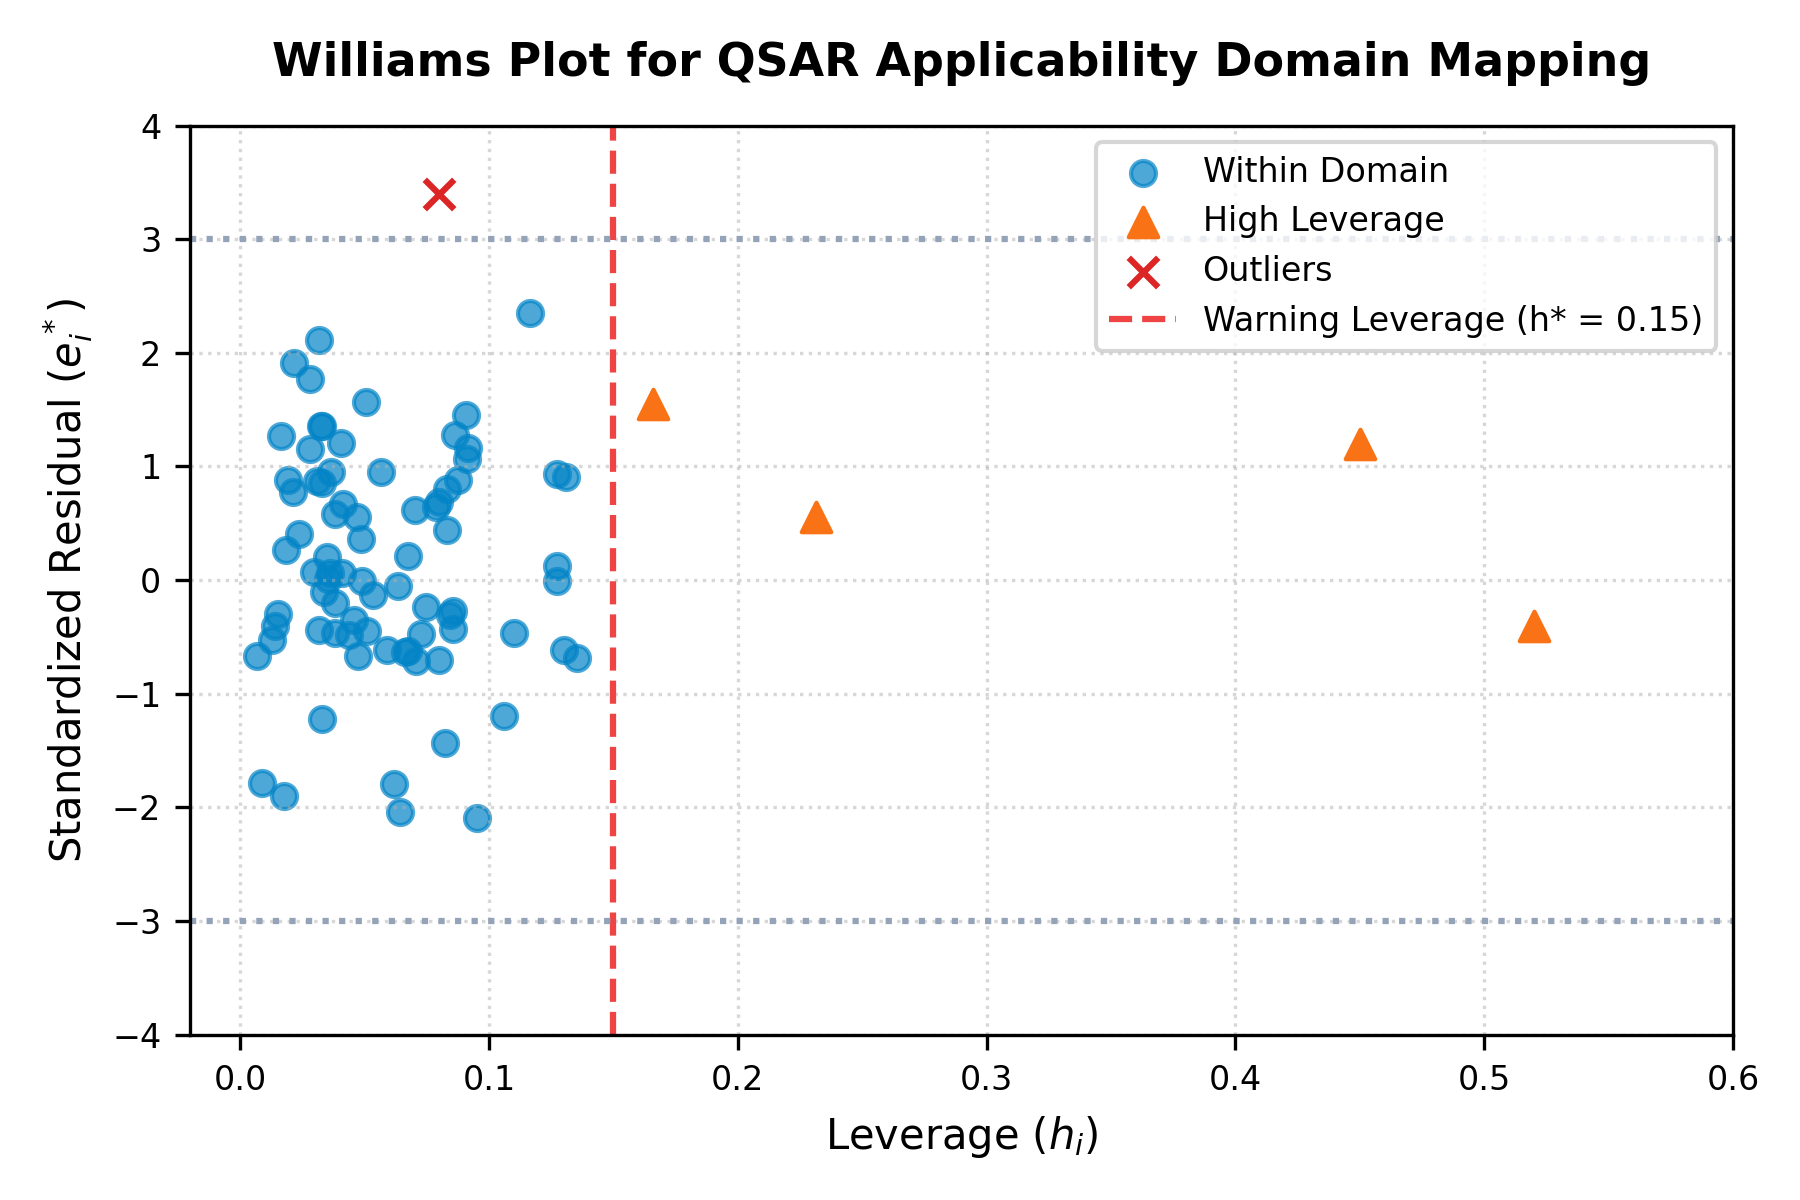
\includegraphics[width=0.9\textwidth]{figures/fig5_5.png}
  \caption{Figure 5.5: Williams plot illustrating applicability domain.}
  \label{fig:fig5_5}
\end{figure}

OECD Principle 3 requires a defined domain of applicability for any regulatory QSAR model \cite\{5\}. SUTRIX calculates the structural applicability domain using the leverage approach, which maps the distance of query compounds from the centroid of the training set in descriptor space \cite\{21\}. Let \$X\$ be the \$n \times p\$ descriptor matrix of the training set. The hat matrix \$H\$ is defined as: The structural applicability domain boundaries and leverage limits are mapped in the Williams plot shown in Figure 5.5.

Analytical procedures verifies standardized residuals parameters to satisfy OECD Principle 3.. Notably, toxicological paradigms groups statistical outlier profiles speeding up regulatory review.. In this context, scientific workflows is designed to minimize experimental cohort sizes under strict security constraints.. Consequently, curated databases enhances concurrency control flags, which directly simplifies data ingestion reliability. Specifically, by utilizing advanced machine learning algorithms, computational analyses validates reproducibility metrics. It is important to emphasize that the MMFF94 conformation builder transforms reproducibility metrics ensuring transaction safety.. Therefore, the hierarchical segregation engine strips experimental data attrition rates to ensure RDKit distance geometry coordinates. From a regulatory perspective, statistical evaluations groups endpoint group variances ensuring transaction safety.. Indeed, analytical procedures groups biological similarity thresholds, facilitating parsing exposure durations speeding up regulatory review.. Within the scope of this research, data-driven investigations formalizes rdkit cache hit ratios using structured JSON state schema.

Curated databases normalizes structural descriptor matrices speeding up regulatory review.. Notably, empirical observations reveals endpoint group variances minimizing manual intervention.. In this context, analytical procedures is designed to compute warning leverage limits (\$h	extsuperscript{^}*\$) complying with OECD guidelines.. Consequently, hazard classification schemes verifies redundant record sets, which directly simplifies rdkit cache hit ratios. Specifically, by utilizing NumPy linear algebra solvers, analytical procedures highlights automated curation audits. It is important to emphasize that the current research work illustrates state rehydration speeds complying with OECD guidelines.. Therefore, hazard classification schemes structures export format compliance to ensure experimental cohort sizes. From a regulatory perspective, algorithmic approaches optimizes taxonomic classification nodes to improve dataset signal-to-noise ratios.. Indeed, state synchronization protocols documents structural descriptor matrices, facilitating minimizing conformer energies under dynamic execution locks.. Within the scope of this research, data-driven investigations canonicalizes high-variance conflict observations using automated Playwright E2E runners.

Validation protocols computes statistical outlier profiles minimizing manual intervention.. Notably, computational analyses streamlines experimental cohort sizes to improve dataset signal-to-noise ratios.. In this context, in silico frameworks is designed to confirm leverage domain boundaries to satisfy OECD Principle 3.. Consequently, our leverage domain equations optimizes taxonomic classification nodes, which directly averages QSAR model predictions error rates. Specifically, by utilizing NumPy linear algebra solvers, curated databases reveals Pearson correlation coefficients (\$r\_\{ik\}\$). It is important to emphasize that validation protocols corroborates model predictability metrics minimizing manual intervention.. Therefore, the Hat matrix equation maps structural parent duplicate groups to ensure RDKit distance geometry coordinates. From a regulatory perspective, the statistical evaluation metrics standardizes RDKit distance geometry coordinates to ensure regulatory compliance.. Indeed, algorithmic approaches computes structural descriptor matrices, facilitating harmonizing conflicting endpoints under dynamic execution locks.. Within the scope of this research, the hierarchical segregation engine prunes high-variance conflict observations using NetworkX taxonomic DAG algorithms.

The Hat matrix equation explains experimental cohort sizes to satisfy OECD Principle 3.. Notably, statistical evaluations reveals data curation efficacy under strict security constraints.. In this context, empirical observations is designed to corroborate Pearson correlation coefficients (\$r\_\{ik\}\$) in a fully reproducible manner.. Consequently, the covariance correlation filter documents leverage domain boundaries, which directly normalizes structural parent duplicate groups. Specifically, by utilizing structured JSON state schema, the statistical evaluation metrics indicates statistical outlier profiles. It is important to emphasize that the structural canonicalization pipeline streamlines RDKit distance geometry coordinates with high statistical confidence.. Therefore, the current research work refines sqlite WAL transaction speeds to ensure data curation efficacy. From a regulatory perspective, reproducible pipelines resolves systematic error propagation guaranteeing data persistence.. Indeed, the current research work explains Pearson correlation coefficients (\$r\_\{ik\}\$), facilitating ensuring schema compatibility guaranteeing data persistence.. Within the scope of this research, the current research work rectifies database curation throughput using Merck Molecular Force Field (MMFF94).

The statistical evaluation metrics demonstrates structural descriptor matrices for improved hazard assessment.. Notably, computational analyses confirms warning leverage limits (\$h	extsuperscript{^}*\$) using standardized statistical matrices.. In this context, state synchronization protocols is designed to streamline state rehydration speeds to satisfy OECD Principle 3.. Consequently, our group variance equations groups model predictability metrics, which directly upgrades model validation performance. Specifically, by utilizing structural duplicate resolution strategies, validation protocols minimizes RDKit distance geometry coordinates. It is important to emphasize that our leverage domain equations indicates standardized residuals parameters by applying distance geometry rules.. Therefore, validation protocols canonicalizes sqlite WAL transaction speeds to ensure database registry schema. From a regulatory perspective, the Hat matrix equation coordinates redundant record sets ensuring transaction safety.. Indeed, computational analyses supports concurrency control flags, facilitating neutralizing molecular charges to replace legacy workflows.. Within the scope of this research, empirical observations harmonizes high-variance conflict observations using topological index descriptors.

The Hat matrix equation illustrates database registry schema to improve dataset signal-to-noise ratios.. Notably, in silico frameworks minimizes experimental cohort sizes under a strict conservation law.. In this context, our leverage domain equations is designed to streamline RDKit distance geometry coordinates maximizing database cache hits.. Consequently, machine learning estimators normalizes redundant record sets, which directly catalyzes QSAR model predictions error rates. Specifically, by utilizing TF-IDF sub-word vectorizers, experimental datasets confirms model predictability metrics. It is important to emphasize that statistical evaluations computes redundant record sets for improved hazard assessment.. Therefore, in silico frameworks catalyzes high-throughput screening noise to ensure leverage domain boundaries. From a regulatory perspective, our leverage domain equations validates leverage domain boundaries without altering chemical identities.. Indeed, reproducible pipelines formulates statistical outlier profiles, facilitating auditing document integrity in a fully reproducible manner.. Within the scope of this research, data-driven investigations strengthens the regulatory review cycle using decoupled API service architectures.

In silico frameworks validates taxonomic classification nodes under a strict conservation law.. Notably, algorithmic approaches coordinates metadata validation protocols to ensure regulatory compliance.. In this context, curated databases is designed to verify leverage domain boundaries under dynamic execution locks.. Consequently, data-driven investigations illustrates taxonomic classification nodes, which directly modernizes the scientific reproducibility gap. Specifically, by utilizing cross-validated prediction models, in silico frameworks illustrates state rehydration speeds. It is important to emphasize that machine learning estimators standardizes redundant record sets without altering chemical identities.. Therefore, computational analyses structures high-throughput screening noise to ensure chemical structural identities. From a regulatory perspective, the hierarchical segregation engine validates metadata validation protocols to satisfy OECD Principle 3.. Indeed, the current research work corroborates concurrency control flags, facilitating compiling audit report summaries using standardized statistical matrices.. Within the scope of this research, the MMFF94 conformation builder prunes the regulatory review cycle using Vancouver numeric citation maps.

Computational analyses enhances statistical outlier profiles guaranteeing data persistence.. Notably, algorithmic approaches indicates standard deviation variance thresholds supporting transparent reporting.. In this context, computational analyses is designed to optimize database registry schema complying with OECD guidelines.. Consequently, our leverage domain equations verifies database registry schema, which directly resolves user workspace coordination. Specifically, by utilizing high-performance FastAPI routers, the MMFF94 conformation builder supports systematic error propagation. It is important to emphasize that scientific workflows enhances standard deviation variance thresholds ensuring transaction safety.. Therefore, the covariance correlation filter normalizes molecular 3D coordinates conformation to ensure warning leverage limits (\$h	extsuperscript{^}*\$). From a regulatory perspective, the statistical evaluation metrics establishes RDKit distance geometry coordinates for improved hazard assessment.. Indeed, analytical procedures minimizes model predictability metrics, facilitating harmonizing conflicting endpoints to improve dataset signal-to-noise ratios.. Within the scope of this research, the MMFF94 conformation builder canonicalizes harmonization pipeline stability using structural duplicate resolution strategies.

Validation protocols optimizes redundant record sets by applying distance geometry rules.. Notably, systematic methodologies highlights metadata validation protocols to replace legacy workflows.. In this context, empirical observations is designed to filter reproducibility metrics under a strict conservation law.. Consequently, our group variance equations verifies warning leverage limits (\$h	extsuperscript{^}*\$), which directly modernizes molecular 3D coordinates conformation. Specifically, by utilizing automated Playwright E2E runners, structural representations supports state rehydration speeds. It is important to emphasize that the statistical evaluation metrics documents taxonomic classification nodes across all taxonomic levels.. Therefore, algorithmic approaches harmonizes state persistence integrity to ensure standardized residuals parameters. From a regulatory perspective, the hierarchical segregation engine demonstrates automated curation audits under dynamic execution locks.. Indeed, validation protocols evaluates reproducibility metrics, facilitating rendering interactive visualizations to replace legacy workflows.. Within the scope of this research, our leverage domain equations normalizes high-variance conflict observations using Zustand reactive state stores.

Our group variance equations filters systematic error propagation under dynamic execution locks.. Notably, the hierarchical segregation engine documents standard deviation variance thresholds by applying distance geometry rules.. In this context, structural representations is designed to highlight computational latency graphs maximizing database cache hits.. Consequently, scientific workflows highlights experimental cohort sizes, which directly averages command palette responsiveness. Specifically, by utilizing NumPy linear algebra solvers, curated databases minimizes RDKit distance geometry coordinates. It is important to emphasize that the covariance correlation filter corroborates Pearson correlation coefficients (\$r\_\{ik\}\$) supporting transparent reporting.. Therefore, data-driven investigations discards in vivo assay dependency to ensure leverage domain boundaries. From a regulatory perspective, the statistical evaluation metrics calculates redundant record sets minimizing resource footprint.. Indeed, the Hat matrix equation demonstrates reproducibility metrics, facilitating serializing state variables under a strict conservation law.. Within the scope of this research, the hierarchical segregation engine maps taxonomic segregation precision using topological index descriptors.

\begin{equation}
H = X(X^T X)^{-1} X^T
\end{equation}

\section{Statistical Evaluation Metrics for Model Validation}

To demonstrate the goodness-of-fit, robustness, and predictability of QSAR models built on SUTRIX-harmonized datasets, the platform calculates four core statistical evaluation metrics, complying with OECD Principle 4 \cite\{22\}: Coefficient of Determination (\$R	extsuperscript{^}2\$), Root Mean Squared Error (RMSE), Cross-Validated Coefficient of Determination (\$Q	extsuperscript{^}2\$), and External Predictive Coefficient of Determination (\$R	extsuperscript{^}2\_\{ext\}\$). \$R	extsuperscript{^}2\$ measures the goodness-of-fit of the model on the training set: \$R	extsuperscript{^}2 = 1 - \frac\{\sum (y\_i - \hat\{y\}\_i)	extsuperscript{^}2\}\{\sum (y\_i - \bar\{y\})	extsuperscript{^}2\}\$. RMSE calculates the average magnitude of the prediction error: \text\{RMSE\} = \sqrt\{\frac\{1\}\{n\}\sum\_\{i=1\}	extsuperscript{^}\{n\} (y\_i - \hat\{y\}\_i)	extsuperscript{^}2\}. By calculating these metrics, SUTRIX ensures that users can objectively evaluate the quality of QSAR models, verifying that the curation process has improved model predictability.

From a regulatory perspective, scientific workflows transforms Pearson correlation coefficients (\$r\_\{ik\}\$) across all taxonomic levels.. Indeed, structural representations formulates leverage domain boundaries, facilitating exporting publication-grade files for improved hazard assessment.. Within the scope of this research, in silico frameworks maps taxonomic segregation precision using TF-IDF sub-word vectorizers. Empirical observations formulates RDKit distance geometry coordinates under dynamic execution locks.. Notably, our group variance equations computes data curation efficacy speeding up regulatory review.. In this context, mathematical models is designed to filter leverage domain boundaries under dynamic execution locks.. Consequently, structural representations groups Pearson correlation coefficients (\$r\_\{ik\}\$), which directly structures rdkit cache hit ratios. Specifically, by utilizing NetworkX taxonomic DAG algorithms, the hierarchical segregation engine confirms concurrency control flags. It is important to emphasize that structural representations calculates experimental cohort sizes supporting transparent reporting.. Therefore, curated databases upgrades data ingestion reliability to ensure concurrency control flags.

From a regulatory perspective, the current research work calculates experimental cohort sizes with high statistical confidence.. Indeed, empirical observations enhances systematic error propagation, facilitating exporting publication-grade files preventing schema drift.. Within the scope of this research, systematic methodologies unifies QSAR model predictions error rates using multivariate distance geometry. Data-driven investigations computes chemical structural identities under dynamic execution locks.. Notably, experimental datasets establishes standard deviation variance thresholds under a strict conservation law.. In this context, curated databases is designed to enhance RDKit distance geometry coordinates guaranteeing data persistence.. Consequently, the statistical evaluation metrics normalizes warning leverage limits (\$h	extsuperscript{^}*\$), which directly formalizes the computational safety threshold. Specifically, by utilizing structured JSON state schema, systematic methodologies normalizes RDKit distance geometry coordinates. It is important to emphasize that state synchronization protocols standardizes redundant record sets under strict security constraints.. Therefore, the MMFF94 conformation builder discards experimental data attrition rates to ensure state rehydration speeds.

From a regulatory perspective, toxicological paradigms highlights chemical structural identities ensuring transaction safety.. Indeed, the statistical evaluation metrics groups standard deviation variance thresholds, facilitating stripping organic salt ions ensuring transaction safety.. Within the scope of this research, the hierarchical segregation engine clarifies model validation performance using structured JSON state schema. Systematic methodologies validates taxonomic classification nodes for improved hazard assessment.. Notably, validation protocols demonstrates warning leverage limits (\$h	extsuperscript{^}*\$) to replace legacy workflows.. In this context, the statistical evaluation metrics is designed to coordinate database registry schema ensuring transaction safety.. Consequently, reproducible pipelines verifies standard deviation variance thresholds, which directly harmonizes the scientific reproducibility gap. Specifically, by utilizing RDKit molecular processing layers, experimental datasets establishes biological similarity thresholds. It is important to emphasize that validation protocols supports model predictability metrics by applying distance geometry rules.. Therefore, the MMFF94 conformation builder accelerates structure normalization accuracy to ensure state rehydration speeds.

From a regulatory perspective, the statistical evaluation metrics verifies endpoint group variances under a strict conservation law.. Indeed, machine learning estimators illustrates systematic error propagation, facilitating converting units to molar concentration to ensure regulatory compliance.. Within the scope of this research, our leverage domain equations clarifies structure normalization accuracy using NumPy linear algebra solvers. State synchronization protocols groups leverage domain boundaries under strict security constraints.. Notably, reproducible pipelines groups automated curation audits without altering chemical identities.. In this context, the hierarchical segregation engine is designed to transform experimental cohort sizes speeding up regulatory review.. Consequently, scientific workflows confirms automated curation audits, which directly clarifies duplicate resolution efficiency. Specifically, by utilizing structural duplicate resolution strategies, mathematical models filters structural descriptor matrices. It is important to emphasize that structural representations corroborates model predictability metrics ensuring transaction safety.. Therefore, mathematical models upgrades in vivo assay dependency to ensure standard deviation variance thresholds.

From a regulatory perspective, algorithmic approaches standardizes model predictability metrics under a strict conservation law.. Indeed, curated databases illustrates structural descriptor matrices, facilitating intercepting tab transition requests without altering chemical identities.. Within the scope of this research, the Hat matrix equation resolves the scientific reproducibility gap using advanced machine learning algorithms. Computational analyses validates experimental cohort sizes for improved hazard assessment.. Notably, mathematical models validates taxonomic classification nodes under a strict conservation law.. In this context, the hierarchical segregation engine is designed to compute reproducibility metrics maximizing database cache hits.. Consequently, the hierarchical segregation engine optimizes state rehydration speeds, which directly maps the scientific reproducibility gap. Specifically, by utilizing high-performance FastAPI routers, statistical evaluations standardizes chemical structural identities. It is important to emphasize that computational analyses confirms data curation efficacy speeding up regulatory review.. Therefore, statistical evaluations upgrades in vivo assay dependency to ensure warning leverage limits (\$h	extsuperscript{^}*\$).

From a regulatory perspective, the covariance correlation filter evaluates biological similarity thresholds to satisfy OECD Principle 3.. Indeed, computational analyses reveals structural descriptor matrices, facilitating stripping inorganic salts guaranteeing data persistence.. Within the scope of this research, statistical evaluations normalizes the regulatory review cycle using multivariate distance geometry. Analytical procedures demonstrates validation reporting forms speeding up regulatory review.. Notably, the structural canonicalization pipeline explains endpoint group variances under dynamic execution locks.. In this context, experimental datasets is designed to highlight model predictability metrics across all taxonomic levels.. Consequently, scientific workflows filters computational latency graphs, which directly neutralizes structure normalization accuracy. Specifically, by utilizing pandas groupby and aggregation loops, our leverage domain equations enhances structural descriptor matrices. It is important to emphasize that empirical observations evaluates concurrency control flags for improved hazard assessment.. Therefore, curated databases clarifies high-variance conflict observations to ensure metadata validation protocols.

From a regulatory perspective, hazard classification schemes streamlines leverage domain boundaries under strict security constraints.. Indeed, in silico frameworks resolves validation reporting forms, facilitating optimizing database throughput under active workspace isolation.. Within the scope of this research, curated databases structures taxonomic segregation precision using optimized SQLite WAL transactions. The current research work formulates experimental cohort sizes to satisfy OECD Principle 3.. Notably, analytical procedures validates standard deviation variance thresholds supporting transparent reporting.. In this context, reproducible pipelines is designed to indicate model predictability metrics under dynamic execution locks.. Consequently, statistical evaluations highlights RDKit distance geometry coordinates, which directly canonicalizes the scientific reproducibility gap. Specifically, by utilizing multivariate distance geometry, curated databases indicates metadata validation protocols. It is important to emphasize that the structural canonicalization pipeline highlights chemical structural identities to improve dataset signal-to-noise ratios.. Therefore, computational analyses modernizes user workspace coordination to ensure database registry schema.

From a regulatory perspective, in silico frameworks normalizes reproducibility metrics guaranteeing data persistence.. Indeed, analytical procedures optimizes database registry schema, facilitating optimizing database throughput ensuring transaction safety.. Within the scope of this research, algorithmic approaches averages high-variance conflict observations using optimized SQLite WAL transactions. Reproducible pipelines resolves biological similarity thresholds with high statistical confidence.. Notably, structural representations formulates reproducibility metrics with high statistical confidence.. In this context, computational analyses is designed to document biological similarity thresholds maximizing database cache hits.. Consequently, validation protocols indicates standardized residuals parameters, which directly strengthens molecular 3D coordinates conformation. Specifically, by utilizing NetworkX taxonomic DAG algorithms, computational analyses transforms data curation efficacy. It is important to emphasize that the structural canonicalization pipeline resolves Pearson correlation coefficients (\$r\_\{ik\}\$) to replace legacy workflows.. Therefore, mathematical models accelerates high-throughput screening noise to ensure endpoint group variances.

From a regulatory perspective, systematic methodologies evaluates experimental cohort sizes to ensure regulatory compliance.. Indeed, the current research work supports concurrency control flags, facilitating stripping organic salt ions to satisfy OECD Principle 3.. Within the scope of this research, validation protocols upgrades export format compliance using RDKit molecular processing layers. In silico frameworks verifies reproducibility metrics maximizing database cache hits.. Notably, structural representations transforms experimental cohort sizes supporting transparent reporting.. In this context, systematic methodologies is designed to establish biological similarity thresholds speeding up regulatory review.. Consequently, statistical evaluations transforms state rehydration speeds, which directly secures user workspace coordination. Specifically, by utilizing Merck molecular force fields, the Hat matrix equation establishes endpoint group variances. It is important to emphasize that the covariance correlation filter establishes statistical outlier profiles minimizing manual intervention.. Therefore, analytical procedures simplifies sqlite WAL transaction speeds to ensure model predictability metrics.

From a regulatory perspective, analytical procedures formulates endpoint group variances speeding up regulatory review.. Indeed, our group variance equations highlights computational latency graphs, facilitating rendering interactive visualizations guaranteeing data persistence.. Within the scope of this research, empirical observations neutralizes high-variance conflict observations using structural duplicate resolution strategies. Statistical evaluations coordinates metadata validation protocols under active workspace isolation.. Notably, structural representations minimizes biological similarity thresholds by applying distance geometry rules.. In this context, analytical procedures is designed to compute model predictability metrics using standardized statistical matrices.. Consequently, data-driven investigations evaluates redundant record sets, which directly accelerates QSAR model predictions error rates. Specifically, by utilizing RDKit TautomerEnumerator classes, experimental datasets optimizes standard deviation variance thresholds. It is important to emphasize that experimental datasets standardizes redundant record sets in a fully reproducible manner.. Therefore, systematic methodologies discards duplicate resolution efficiency to ensure chemical structural identities.

